\documentclass[10pt,twoside]{article}

%
% Use droid mono for fixed-width font
%
\usepackage[defaultmono,scale=0.8]{droidmono}
\usepackage{amsmath,amssymb,amsthm}
\usepackage[subsection]{algorithm}
\usepackage{algpseudocode}
\renewcommand{\algorithmicrequire}{\textbf{Input:}\,}
\renewcommand{\algorithmicensure}{\textbf{Output:}}
\renewcommand{\algorithmicforall}{\textbf{for each}}
\newcommand{\Input}{\Require}
\newcommand{\Output}{\Ensure}
\newcommand{\ForEach}{\ForAll}
\usepackage{graphicx}
\usepackage{caption}
\usepackage{listings}
\lstset{
%  aboveskip=\bigskipamount,
  basicstyle=\ttfamily\small,
%  belowskip=\bigskipamount,
  frame=single,
  language=Python,
  numbers=left,
  numberstyle=\tiny,
  showstringspaces=false,
  xleftmargin=4pt,
  xrightmargin=4pt
}
\lstnewenvironment{pyoutput}[1][]
{\lstset{aboveskip=-\medskipamount,numbers=none,#1}}
{}



%
% Theorems, Definitions, and Example
%
\theoremstyle{plain}
\newtheorem{theorem}{Theorem}[section]
\newtheorem{lemma}[theorem]{Lemma}
\newtheorem{proposition}[theorem]{Proposition}

\theoremstyle{definition}
\newtheorem{definition}[theorem]{Definition}
\newtheorem{conjecture}[theorem]{Conjecture}
\newtheorem{example}[theorem]{Example}

\numberwithin{equation}{section}
\numberwithin{figure}{section}


%
% Custom operator declarations
%
\DeclareMathOperator{\ZZ}{\mathbb{Z}}
\DeclareMathOperator{\RR}{\mathbb{R}}
\DeclareMathOperator{\CC}{\mathbb{C}}
\DeclareMathOperator{\KK}{\mathbb{C}}
\DeclareMathOperator{\hh}{\mathfrak{h}}
\DeclareMathOperator{\re}{\text{Re}}
\DeclareMathOperator{\im}{\text{Im}}
%\DeclareMathOperator{\PP}{\mathrm{P}}
\newcommand{\PP}[1]{\mathrm{P}^#1 \!}

%
% Make marginpars smaller font
%
\let\oldmarginpar\marginpar
\renewcommand\marginpar[1]{\oldmarginpar[\scriptsize #1]{\scriptsize #1}}

\newcommand{\thchar}[2] {\begin{bmatrix}#1\\#2\end{bmatrix}}
\newcommand{\thcharsm}[2] {\left[ \begin{smallmatrix} #1 \\ #2 \end{smallmatrix} \right]}

\title{Computing with Riemann Surfaces and Abelian Functions \\ {\small
    General Examination}}

\author{
Chris Swierczewski\\
University of Washington\\
Department of Applied Mathematics}
\date{\today}


%%%%%%%%%%%%%%%%%%%%%%%%%%%%%%%%%%%%%%%%%%%%%%%%%%%%%%%%%%%%%%%%%%%%%%%%%%%%%%%
\begin{document}
%%%%%%%%%%%%%%%%%%%%%%%%%%%%%%%%%%%%%%%%%%%%%%%%%%%%%%%%%%%%%%%%%%%%%%%%%%%%%%%

\maketitle

\begin{abstract}
The goal of my research is to use the theory of Riemann surfaces and
Abelian functions to address different application problems and to
develop the software tools necessary for computing with these objects.

Abelian functions are periodic functions of $n$ complex variables having
$2n$ independent periods. Although Abelian functions first arose in the
study of Abelian integrals, they find application in many fields of
mathematics such as solving non-linear integrable partial differential
equations, complex algebraic geometry, optimization, and more. Algebraic
curves and Riemann surfaces form a natural environment for studying
these functions.

In my general examination, I will present the basic theory and
algorithms involved in computing with these objects, demonstrate the
implementation of these algorithms in the Python software library
``abelfunctions'' I developed, and present my objectives for this
research.
\end{abstract}

%%%%%%%%%%%%%%%%%%%%%%%%%%%%%%%%%%%%%%%%%%%%%%%%%%%%%%%%%%%%%%%%%%%%%%%%%%%%%%%%
\section{Introduction}
%%%%%%%%%%%%%%%%%%%%%%%%%%%%%%%%%%%%%%%%%%%%%%%%%%%%%%%%%%%%%%%%%%%%%%%%%%%%%%%

The Kadomtsev-Petviashvili (KP) equation is a partial differential
equation used to describe the surface height of a two-dimensional
periodic shallow water wave. Depending on certain physical
considerations [XXX], which we will ignore, one can derive either of the
following two equations
\begin{align}
  \left(-4u_t + 6uu_x + u_{xxx}\right)_x + 3\sigma^2 u_{yy} = 0, \quad
  \sigma^2 = -1, \label{eqn: KP1} \\
  \left(-4u_t + 6uu_x + u_{xxx}\right)_x + 3\sigma^2 u_{yy} = 0, \quad
  \sigma^2 = +1. \label{eqn: KP2}
\end{align}
where $u(x,y,t)$ is the surface height as a function of position $(x,y)$
and time $t$. In the sequel we do not rely on this distinction and we
simply refer to the ``KP equation''.

The KP equation admits a large family of quasiperiodic solutions of the
form
\begin{equation} \label{eqn: kpsol}
  u(x,y,t) = 2 \partial_x^2 \log \theta(Ux+Vy+Wt+z_0, \Omega) + c,
\end{equation}
where $\theta$ is the Riemann theta function.

\begin{definition} \label{def: riemanntheta}
  The {\bf Riemann theta function} $\theta: \CC^g \times \hh_g \to \CC$
  is defined in terms of its Fourier series:
  \begin{equation} \label{eqn: riemanntheta}
    \theta(z,\Omega) = \sum_{n \in \ZZ^g}
    e^{2 \pi i \left( \tfrac{1}{2} n \cdot \Omega n + n \cdot z \right)}.
  \end{equation}
  This function converges absolutely and uniformly on compact sets in
  $\CC^g \times \hh_g$ where $\hh_g$ is the space of all {\it ``Riemann
    matrices''} --- complex symmetric matrices with positive definite
  imaginary part.
\end{definition}

From the definition, we see that the Riemann theta function is periodic
in $z$ with integer periods and quasi-periodic in $z$ in the columns of
$\Omega$. In other words, if $m,n \in \ZZ^g$ then
\begin{equation} \label{eq: quasiperiodicity}
    \theta(z + m + \Omega n, \Omega) =
    e^{-2 \pi i \left( \tfrac{1}{2} n \cdot \Omega n + n \cdot z \right) }
    \theta(z, \Omega).
\end{equation}

A generalization of the Riemann theta function, involving a non-integer
shift in some of its arguments, is referred to as the Riemann theta
function with characteristics.

\begin{definition} \label{def: thetachar}
Let $\alpha,\beta \in [0,1)^{g}$. The {\bf Riemann theta function with
characteristic $\thcharsm{\alpha}{\beta}$} is defined as
\begin{align*}
  \theta\thchar{\alpha}{\beta}(z, \Omega) &=
  \sum_{n \in \mathbb{Z}^g}
  e^{2 \pi i \left( \tfrac{1}{2} (n+\alpha) \cdot \Omega (n+\alpha) +
    (n + \alpha) \cdot (z + \beta) \right) } \\
  &=
  e^{2\pi i \left( \tfrac{1}{2} \alpha \cdot \Omega \alpha +
    \alpha \cdot (z + \beta) \right)}
  \theta(z + \Omega \alpha + \beta, \Omega).
\end{align*}
\end{definition}

Note that $\theta \thcharsm{0}{0}(z,\Omega) = \theta(z,\Omega)$. See
\cite{NIST:DLMF,MumfordI07,MumfordII07} for further definitions and
properties of the Riemann theta function.

These soltuions \eqref{eqn: kpsol} are the so-called ``theta function
solutions'' to the KP equation and families of such solutions exist for
every $g > 0$. In fact, the totality of solutions of this form are dense
the space of all periodic solutions to KP \cite{Krichever93}. The
constants $c\in\CC$, $U,V,W,z_0 \in \CC^g$ and $\Omega \in \hh_g$, as
well as the {\it genus} $g$, are determined from a Riemann surface any
such Riemann surface can produce a solution to KP \cite{Dubrovin81}. We
postpone the definition of these constants in terms of known quantities
until more machinery is developed in the following chapters.

In general, periodic solutions to integrable partial differential
equations are {\it Abelian functions}.
\begin{definition} \label{def: abelian-function}
  An {\bf Abelian function} $f : \CC^g \to \CC$ of genus $g \geq 1$ is a
  meromorphic function such that there exists $2g$ vectors
  $w_1,\ldots,w_{2g} \in \CC^g$ linearly independent over the real
  numbers where
  \[
      f(z + w) = f(z)
  \]
  for all $z \in \CC^g$. When $g=1$ these are the {\it elliptic
    functions}. The $g \times 2g$ matrix of column vectors $(w_i)$ is
  called the {\it period matrix} of the $f$.
\end{definition}
Abelian functions first arose from the study of Abelian integrals
\[
    \int_{z_0}^{z_1} \frac{P(z,w)}{Q(z,w)}dz
\]
where $P,Q \in \CC[z,w]$ and $z$ and $w$ are related by an algebraic
equation $f(z,w) = 0$ with $f \in \CC[z,w]$. The Jacobi Inversion
Problem is the problem of inverting such integrals, the solution to
which are Abelian functions.

Riemann theta functions play a central role in the theory of Abelian
functions in that all Abelian functions can be written as a rational
function of the Riemann theta function and its derivatives (such as in
the KP solution above).  The primary focus of study is the method of
computation of these Abelian functions, particularly those arising in
applications.

Abelian functions are applicable in fields other than nonlinear partial
differential equations. For example, they make explicit many
computations such as those in the study of solitary waves, black hole
space-times, and algebraic curves. One example in particular is the
calculation of bitangent lines of plane algebraic curves; useful for
computations in optimization-related fields such as algebraic geometry
and convex optimization. In algebraic geometry, bitangents can represent
smooth complex plane quartic curves as both a symmetric determinant of a
linear form (or, determinantal representation) as well as a sum of three
squares \cite{PSV11}. In convex optimization, bitangents are used to
construct a ``visibility complex'' which, in turn, is used to solve the
shortest path problem in Euclidean space \cite{PocchiolaVegter93}.

\begin{definition} \label{def: bitangent}
  A {\bf bitangent} to a plane algebraic curve $C : f(x,y) = 0, f \in
  \CC[x,y]$ is a line $\mathcal{L} \subset \CC$ that lies tangent to $C$
  at at least two distinct points.
\end{definition}

By Bezout's Theorem, if a curve has a bitangent it necessarily must be
of degree at least four \cite{Bezout1779}. A result of Pl\"{u}cker
determines that a degree four complex curve admits exactly 28 complex
bitangents \cite{Plucker34}. In particular, Pl\"{u}cker showed that the
number of real bitangents of any real quartic must be 28, 16, or fewer
than 9. The connection between Riemann theta functions and the bitangent
lines of smooth quartics was known to Riemann \cite{Riemann76,Baker97}
and, in fact, can be computed using the tools developed in this
research. See Figure \ref{fig: edge} for an example.

%!!!!!!!!!!!!!!!!
%!!!!!!!!!!!!!!!!
\marginpar{Note: Figure \ref{fig: edge} will be replaced with the one
  generated by abelfunctions once I have it working properly again /
  once I find the image on my computer.}
%!!!!!!!!!!!!!!!!
%!!!!!!!!!!!!!!!!

\begin{figure}[t]
  \centering
  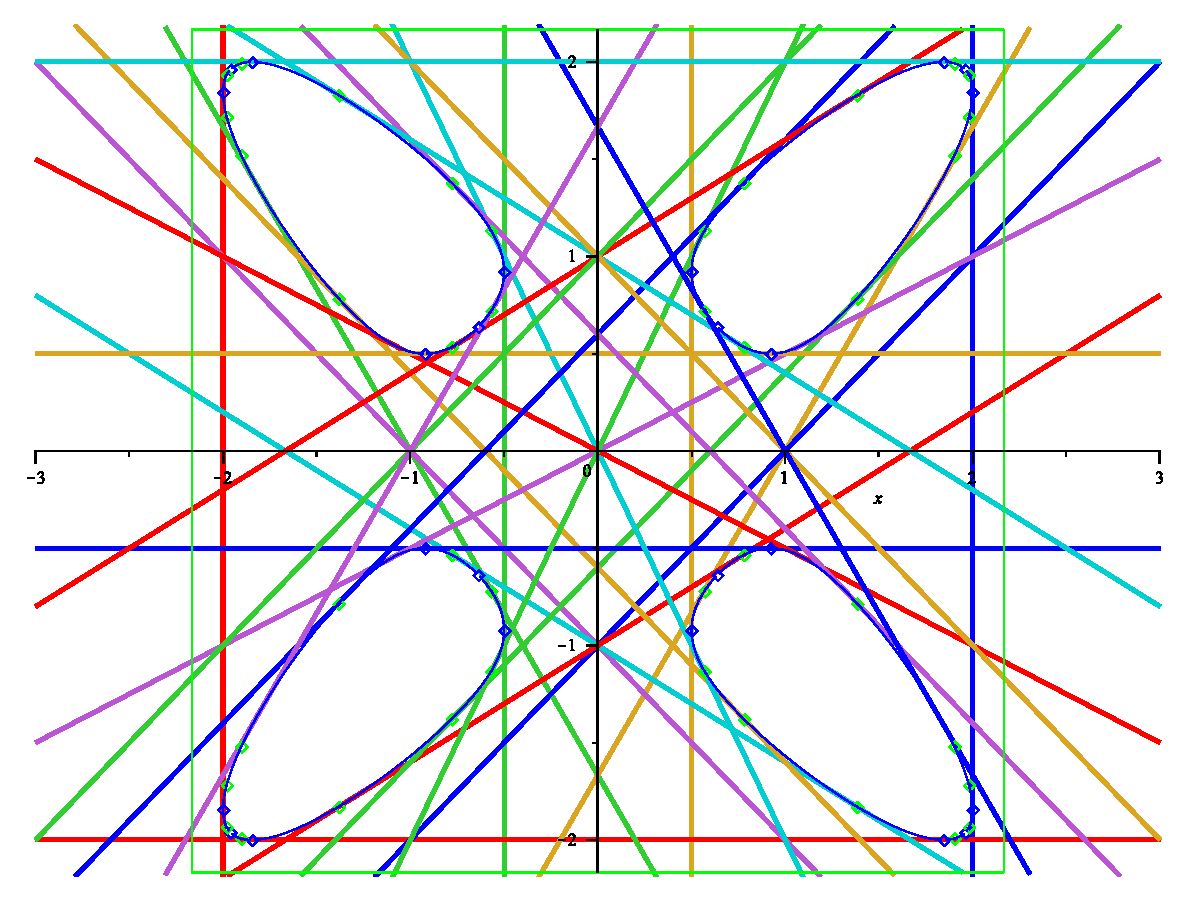
\includegraphics[width=0.8\textwidth]{images/edgequartic}
  \caption{The real graph of the Edge Quartic $C: f(x,y) = 25(x^4+y^4+1)
    - 34(x^2y^2+x^2+y^2) = 0$ and its 28 real bitangents. Note that four
    of them lie tangent $C$ at infinity. These lines were computed using
    the Riemann theta function.}
  \label{fig: edge}
\end{figure}

Finally, Riemann theta functions and algebraic curves can be used to
compute linear matrix representations of algebraic curves. A theorem
from classical algebraic geometry states that every homogenous
polynomial $f \in P^2\CC[x_0,x_1,x_2]$ can be written in the form
\[
   f(x_0,x_1,x_2) = \text{det}
   \left( A x_0 + B x_1 + C x_2 \right),
\]
where $A,B,C$ are symmetric complex matrices which can be efficiently
computed using Riemann theta functions. Furthermore, when the polynomial
has real coefficients then $A,B,C$ are symmetric real matrices and such
representations are important in the study of spectrahedra --- the
solution spaces of semidefinite programs \cite{PSV10}.

The purpose of my research is to develop efficient and performant
algorithms for computing with Abelian functions on Riemann surfaces. The
computational tools developed in this research program have far-reaching
and varied applications.


%%%%%%%%%%%%%%%%%%%%%%%%%%%%%%%%%%%%%%%%%%%%%%%%%%%%%%%%%%%%%%%%%%%%%%%%%%%%%%%%
\section{Complex Algebraic Geometry}
%%%%%%%%%%%%%%%%%%%%%%%%%%%%%%%%%%%%%%%%%%%%%%%%%%%%%%%%%%%%%%%%%%%%%%%%%%%%%%%

This section serves as a brief introduction to the theory of complex
algebraic curves. Primary references are \cite{Ueno97,Griffiths89}.

%..............................................................................
\subsection{The Projective Line}
%..............................................................................

The primary motivation behind complex projective geometry is to make concrete
the way in which we analyze the behavior of functions, such as
polynomials, at infinity without having to resort to techniques separate
from those used at finite points. For example, in applications we may
need to integrate a differential along a path on an algebraic curve
going to infinity. Knowing the geometry of the curve at infinity makes
such an operation computationally feasible.

In fact, anyone with an elementary complex analysis background has seen
an example of projective geometry. The Riemann sphere is the complex
plane $\CC$ with a ``point at infinity'' added. Let $z$ denote the
coordinate in $\CC$ (i.e., the point $z=0$ represents the origin of the
complex plane). In order to discuss the point at infinity we introduce
the coordinate $w = 1/z$. The analysis of some function at $\infty$ is
equivalent to rewriting the problem in terms of the coordinate $w$ and
examining its behavior in a neighborhood of $w=0$. This explains why,
for example, the exponential function
\[
    e^z = \sum_{n=0}^\infty z^n / n!,
\]
though entire in the complex plane, has an essential singularity on the
Riemann sphere since the exponential function in the coordinate $w$
centered at $w=0$ is expressed by the series
\[
    \sum_{n=0}^\infty \frac{w^{-n}}{n!}.
\]

This point at infinity is not rigorously defined because it does not
make sense to {\it equate} $z=\infty$. The definition of the Riemann
sphere is made explicit by the following construction: consider the set
$U = \CC^2 - \{(0,0)\}$. Define the equivalence relation
\[
    (a_0, a_1) \sim (\lambda a_0, \lambda a_1),
    \quad \forall \lambda \in \CC - \{0\}.
\]
Thus two points $(a_0,a_1)$ and $(b_0,b_1)$ in $U$ are considered the
same if the ratios $a_0 : a_1$ and $b_0 : b_1$ are equal. The set of all
points $(b_0,b_1)$ equal to $(a_0,a_1)$ is called the {\it equivalence
  class} of $(a_0,a_1)$ and the {\it complex projective line} $\PP{1}\CC$
is the set of all such equivalence classes. That is,
\[
    \PP{1}\CC := \CC^2 / \sim.
\]
The equivalence class of $(a_0,a_1)$, called a ``point'' in $\PP{1}\CC$,
is written $(a_0 : a_1) \in \PP{1}\CC$. $\PP{1}\CC$ is precisely the
Riemann sphere. To see this, consider the two subsets
\begin{align*}
    U_0 &= \{ (a_0 : a_1) \in \PP{1}\CC \; | \; a_0 \neq 0 \}, \\
    U_1 &= \{ (a_0 : a_1) \in \PP{1}\CC \; | \; a_1 \neq 0 \}.
\end{align*}
For any $(a_0 : a_1) \in U_0$ we have, by the equivalence property,
\[
    (a_0 : a_1) = (1 : a_1/a_0) = (1 : a).
\]
Similarly, $(b_0 : b_1) = (b : 1)$ for every point in $U_1$. Every point
in the intersection $U_0 \cap U_1$ can be written in either of these two
forms. Each of these subspaces are isomorphic to $\CC$ since the maps
\begin{align*}
  \phi_0 : U_0 \to \CC,
  \quad
  \phi_0 \left( (a_0 : a_1) \right) = a_1 / a_0,
  & \quad \text{ and } \\
  \phi_1 : U_1 \to \CC,
  \quad
  \phi_1 \left( (a_0 : a_1) \right) = a_0 / a_1, &
\end{align*}
are continuous bijections with inverses
\begin{gather}
  \phi^{-1}_0(a) = (1 : a), \\
  \phi^{-1}_1(b) = (b : 1).
\end{gather}
Finally, note that $(0 : 1)$ is the only projective point in $U_1$ which
is not in $U_0$. Therefore, we identify $U_0$ with the complex plane (in
the coordinate $z$) and the point $P_\infty = (0 : 1)$ with the point at
infinity and set
\begin{equation} \label{eqn: projective-line}
  \PP{1}\CC = U_0 \cup \{ (0 : 1) \} \cong \CC \cup P_\infty.
\end{equation}

Indeed $P_\infty$ is considered the point at infinity on the Riemann
sphere for if one considers the image of $(0 : 1)$ under $\phi_0$,
though undefined since $(0:1) \not \in U_0$, it maps to $z = 1 / 0$
``='' $\infty$. Again, this does not make sense without the complex
projective space construction above but is merely used to illustrate the
point. The coordinate transformation from $z$ to $w$ at the beginning of
this section is equivalent to identifying $U_1$ with the complex plane
$\CC$ and $\{(1 : 0)\}$ with the point at infinity, instead.

%------------------------------------------------------------------------------
\subsection{The Projective Plane}
%------------------------------------------------------------------------------

The natural environment we use in the sequel is not the complex
projective line but the complex projective plane. In this section we
construct the projective plane and examine its geometric properties. The
construction is similar to that of the projective line.

Let $U = \CC^3 - \{(0,0,0)\}$. Following the strategy of the previous
section, consider the set of all ratios $(a_0 : a_1 : a_2)$, that is,
the collection of all equivalence classes under the equivalence relation
$(a_0 : a_1 : a_2) \sim (\lambda a_0 : \lambda a_1 : \lambda a_2),
\forall \lambda \in \CC - \{0\}$. The space of all such equivalence
classes is called the two-dimensional complex projective space or {\it
  the projective plane} and is denoted $\PP{2}\CC$.

Define the subsets $U_0,U_1,U_2$ by
\[
    U_j = \{ (a_0 : a_1 : a_2) \in \PP{2}\CC \; | \; a_j \neq 0 \},
\]
and note that all $(a_0 : a_1 : a_2) \in U_0$ satisfy $(a_0 : a_1 : a_2)
= (1 : a_1/a_0 : a_2/a_0)$. We define the bijective mapping
\begin{gather*}
    \phi_0 : U_0 \to \CC^2, \\
    \phi_0 \left( (a_0 : a_1 : a_2) \right)
    =
    \left( \frac{a_1}{a_0}, \frac{a_2}{a_0} \right), \\
    \phi_0^{-1} \left( (x,y) \right)
    =
    (1 : x : y).
\end{gather*}
The mappings $\phi_1$ and $\phi_2$ are similarly defined on $U_1$ and
$U_2$, respectively. Therefore, we can identify $U_0$ with the complex
plane $\CC^2$.

Consider the space $U_0^c = \PP{2}\CC - U_0$. By definition, every point
in $U_0^c$ is of the form $(0 : a_1 : a_2)$. By definition, every point
in $U_0^c$ determines a point on the complex projective line
$\PP{1}\CC$. The converse is true as well, resulting in the bijection
\[
    (0 : a_1 : a_2) \in \PP{2}\CC
    \; \leftrightarrow \;
    (a_1 : a_2) \in \PP{1}\CC.
\]
By identifying $U_0^c$ with $\PP{1}\CC$ we may write
\begin{equation} \label{eqn: proejctive-plane}
  \PP{2}\CC = U_0 \cup U_0^c \cong \CC^2 \cup \PP{1}\CC
\end{equation}
where $U_0^c \cong \PP{1}\CC$ is called the {\it line at infinity},
denoted $l_\infty$, and $U_0 \cong \CC^2$ is called the {\it complex
  affine plane}. We may also identify the complex affine plane with the
sets $U_1$ or $U_2$ and the line at infinity with their complements.

We saw a natural geometric interpretation of $\PP{1}\CC$ in the previous
section. Does such an interpretation exist for $\PP{2}\CC$? Consider a line
in the complex affine plane $\CC^2$ which can be written in the form
\[
    \alpha + \beta x + \gamma y = 0,
    \quad \text{where }
    (\beta,\gamma) \neq 0, \alpha, \beta, \gamma \in \CC.
\]
Using the inverse mapping $\phi_0^{-1}$ on $\CC^2$ we have
\[
    x = \frac{x_1}{x_0} \text{ and } y = \frac{x_2}{x_0},
\]
where $(x_0 : x_1 : x_2)$ are the coordinates of $\PP{2}\CC$, and we get
the line
\[
    \alpha x_0 + \beta x_1 + \gamma x_2 = 0.
\]
This equation, called the {\it homogenization} of the affine curve,
makes sense in all of $\PP{2}\CC$. Setting $x_0 = 1$ gives the original
affine line. On the other hand, setting $x_0 = 0$ gives the equation
\[
    \beta x_1 + \gamma x_2 = 0,
\]
which is the equation of the line in $l_\infty$. However, this implies
$x_1 / x_2 = - \gamma / \beta$. Hence the projective point $(0 : -\gamma
: \beta)$ satisfies the equation
\[
    \alpha x_0 + \beta x_1 + \gamma x_2 = 0
\]
and is, in fact, the only projective point in $l_\infty$ on the line.

This means that the line ``intersects'' $l_\infty$ at the point $(0 :
-\gamma : \beta)$ and that this intersection point depends only on the
slope of the affine portion of the line. Hence, the line at infinity has
the geometric meaning that each point on it is the intersection point of
an entire family of parallel lines in $\CC^2$. This leads to a
generalization of a theorem from classical planar geometry: {\it any
  two, distinct lines in $\PP{2}\CC$ intersect at exactly one point}.

%------------------------------------------------------------------------------
\subsection{Projective Plane Curves} \label{sec: projective-plane-curves}
%------------------------------------------------------------------------------

The set of all points $(x_0, x_1, x_2)$ satisfying
\[
    \alpha x_0 + \beta x_1 + \gamma x_2 = 0
\]
is called a projective line and is a simple example of a projective
algebraic curve (of degree one). In this section we introduce various
properties of general projective curves.

An {\it complex plane algebraic curve} is the zero locus of the
homogenization of a polynomial $f \in \CC[x,y]$. That is, given a
polynomial $f(x,y) = \alpha_n(x) y^n + \alpha_{n-1}(x)y^{n-1} + \cdots +
\alpha_0(x)$ its homogenization is the polynomial $F \in
\PP{2}\CC[x_0,x_1,x_2]$ where
\[
    F(x_0,x_1,x_2) = x_0^d f(x_1/x_0,x_2/x_0).
\]
where $d$ is the degree of $F$. The homogeneity of $F$ means that we can
write
\[
    F(x_0,x_1,x_2) = \sum_{i+j+k=d} \alpha_{ijk} x_0^i x_1^j x_2^k.
\]

In terms of the projective polynomial $F$, its affine part can be
written $f(x,y) = F(1,x,y)$. As in the case of a projective line, $f$
can be thought of as a projection of the polynomial $F$ onto $\CC^2$ and
there is always a one-to-one correspondence between an affine polynomial
and its homogenization. Therefore, a {\it complex plane algebraic curve}
is the set
\[
  C = \left\{
  (x_0 : x_1 : x_2) \in \PP{2}\CC : F(x_0,x_1,x_2) = 0
  \right\}.
\]

Important to the study of projective curves, and specifically in the
computational work described here, are singular points.
\begin{definition} \label{def: singular-point}
  A point $a = (a_0 : a_1 : a_2) \in C$ is a {\bf singular point of
    $C$}, or a {\it multiple point of $C$}, if
  \[
      \left(
        \frac{\partial F}{\partial x_0},
        \frac{\partial F}{\partial x_1},
        \frac{\partial F}{\partial x_2}
      \right) (a)
      = (0,0,0).
  \]
\end{definition}
Consider the case when $a = (1 : 0 : 0)$ (corresponding to the point
$(0,0)$ in the affine plane $\CC^2$) is a singular point of $F$. The
affine poirtion of the curve is
\[
f(x,y) = \sum_{i+j \geq 2}^d c_{ij} x^iy^j.
\]
Note that the constant term is zero since $(0, 0)$ is a point on the
affine curve and the linear term vanishes since $(0,0)$ is a singular
point. We write
\[
  f(x,y) = f_m(x,y) + f_{m+1}(x,y) + \cdots + f_d(x,y), \quad m \geq 2,
\]
where each $f_n$ is the sum of all terms of $f$ of degree $n$; that is,
terms of the form $c_{ij}x^iy^j$ such that $i+j=n$. The smallest such
$m$ with non-zero term $f_m$ appearing in $f$ is called the {\it
  multiplicity} of the singular point $(1 : 0 : 0)$. Singularities with
multiplicity two are called {\it double points}, those with multiplicity
three are called {\it triple points}, and so on.

The homogeneous term $f_m$ can be factored into linear factors
\[
  f_m(x,y) = \prod_{j=1}^m (\alpha_j x - \beta_j y).
\]
We call the space $f_m(x,y) = 0$ the {\it tangent cone of the plane
  curve $C$} at $a = (1 : 0 : 0)$ consistsing of a finite number of
intersecting lines $L_j : \alpha_j x - \beta_j y$.

When a generic affine point $a = (1 : c : d)$ is a singular point we
write the affine curve in the form
\[
    f(x,y) = \sum_{i+j \geq 2}^d \tilde{c}_{ij} (x-c)^i(y-d)^j
\]
which we can write as a sum of polynomials $g_n(x-c,y-d)$ homogenous in
$x-c$ and $y-d$.

In the case when the singular point $a = (0 : 1 : b) \in l_\infty$ we
repeat the above process with the affine curve
\[
    g(u,v) = \frac{1}{x_1^d} F(x_0, x_1, x_2) = F(u,1,v),
    \quad u = \frac{x_0}{x_1}, v = \frac{x_2}{x_1},
\]
which is a projection of $F$ onto $U_1 \cong \CC$ instead of $U_0$.  We
write $g$ as a sum of terms of the form $g_{ij}u^i(v-b)^j$. Finally, in
the case $a = (0 : 0 : 1) \in l_\infty$ we use the affine curve
\[
    h(w,z) = \frac{1}{x_2^d} F(x_0, x_1, x_2) = F(w,z,1),
    \quad w = \frac{x_0}{x_2}, z = \frac{x_1}{x_2},
\]
and write $h$ as a sum of terms of the form $h_{ij}w^iz^j$.

\begin{example} \label{ex: 2-cubic}
Consider the cubic curve
\[
    C: F(x_0,x_1,x_2) =
    x_0^4 x_2^3 + 2 x_0^3 x_1^3 x_2 - x_1^7
\]
In complex affine space $x_0 = 1$ this curve is
\[
    f(x,y) = F(1,x,y) = y^3 + 2 x^3 y - x^7.
\]
A plot of $f$ for $x,y$ real is shown in Figure \ref{fig: example-cubic}.
For $a = (a_0 : a_1 : a_2)$ we have
\begin{align} \label{eq: singular-conditions}
    \frac{\partial F}{\partial x_0}(a)
    &=
    4 a_{0}^{3} a_{2}^{3} + 6 a_{0}^{2} a_{1}^{3} a_{2}, \notag \\
    \frac{\partial F}{\partial x_1}(a)
    &=
    6 a_{0}^{3} a_{1}^{2} a_{2} - 7 a_{1}^{6}, \notag \\
    \frac{\partial F}{\partial x_2}(a)
    &=
    3 a_{0}^{4} a_{2}^{2} + 2 a_{0}^{3} a_{1}^{3}.
\end{align}

\begin{figure}
  \centering
  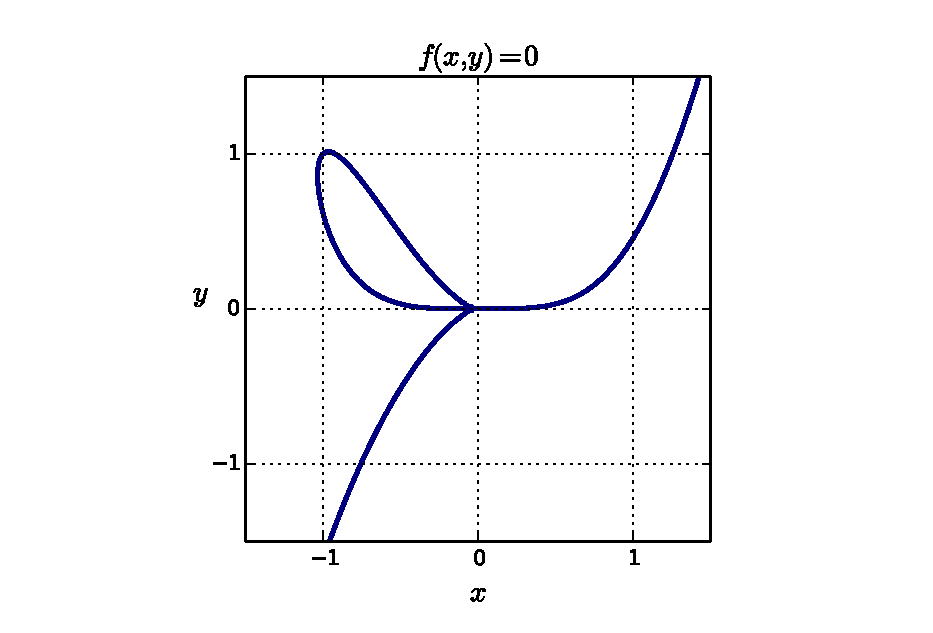
\includegraphics[width=0.9\textwidth]{images/singularities-example.eps}
  \caption{A real plot of the curve $C : f(x,y) = y^3 + 2 x^3 y -
    x^7$. The plot suggests that $(x_0 : x_1 : x_2) = (1 : 0 : 0)$,
    corresponding to $(x,y) = (0,0)$, is a singular point of $C$.}
  \label{fig: example-cubic}
\end{figure}

First, we find the finite singular points of $C$. Setting $a_0=1$ and
solving the above equations for $a_1$ and $a_2$ we see that $p = (1 : 0
: 0)$ is the only finite singular point of $F$. Note that
\begin{gather*}
    f(x,y) = f_3(x,y) + f_4(x,y) + f_7(x,y), \\
    \\
    f_3(x,y) = y^3, \quad
    f_4(x,y) = 2 x^3 y, \quad
    f_7(x,y) = -x^7,
\end{gather*}
and that $f_3$, $f_4$, and $f_7$ are homogeneous of degrees 3, 4, and 7,
respectively. Therefore, $p$ is a singular point of multiplicity 3 with
\[
    f_3(x,y) = y^3 = 0,
\]
as the equation for the tangent cone at $p$. These properties are
suggested by Figure \ref{fig: example-cubic} where, near the point $p$,
the real curve looks like the intersection of three curves well
approximated by the line $y = 0$ near the point $x = 0$.

Setting $a_0 = 0$, the only expression in Equation \eqref{eq:
  singular-conditions} that does not reduce to zero is
\[
    \frac{\partial F}{\partial x_1}((0,a_1,a_2))
    =
    - 7 a_{1}^{6} = 0,
\]
implying that the point $a = (0 : 0 : 1)$ is the only singular point at
infinity. The curve at infinity centered at $(0 : 0 : 1)$ is
\[
    h(w,z) = F(w,z,1) = w^{4} + 2 w^{3} z^{3} - z^{7}.
\]
The order of this singularity is four since this is the degree of the
lowest degree homogeneous term. The tangent cone at $a$ is $g_4(w,z) =
w^4$.
\end{example}


%------------------------------------------------------------------------------
\subsection{Connection to Riemann Surfaces}
%------------------------------------------------------------------------------

There is a close relationship between the study of compact Riemann
surfaces and that of algebraic curves. Recall that a Riemann surface
$X$ is a complex manifold of complex dimension one endowed with
an {\it atlas}: an open covering $\{U_\alpha \}_{\alpha \in A}$ of
$X$ together with a collection of homeomorphisms $\{z_\alpha :
U_\alpha \to \CC\}_{\alpha \in A}$, called {\it local parameters}, such
that every pair of {\it transition functions}
\[
    f_{\beta,\alpha} := z_\beta \circ z_\alpha^{-1} :
    z_\alpha \left( U_\alpha \cap U_\beta \right)
    \to
    z_\beta \left( U_\alpha \cap U_\beta \right),
\]
is holomorphic. The pairs $(U_\alpha, z_\alpha)$ are called {\it
  coordinate charts}. In other words, a Riemann surface is a topological
space such that for all $P \in X$ there is a neighborhood of $P$
homeomorphic to an open subset of the complex plane and one can
analytically continue from any $P \in X$ to any $Q \in X$ via transition
functions.

The Riemann sphere $X = \CC^*$ is an example of a Riemann
surface. Its atlas consists of two coordinate charts $(U_1, z_1)$ and
$(U_2, z_2)$ with
\begin{align*}
    U_1 = \CC, & \quad z_1 = z, \\
    U_2 = \left( \CC - \{0\} \right) \cup \{ \infty \}, & \quad z_2 = 1/z.
\end{align*}
This is a valid atlas since the transition functions
\begin{gather*}
    f_{1,2}, f_{2,1} : \left(\CC - \{0\}\right)
    \to \left(\CC - \{0\}\right) \\
    f_{1,2} = z_1 \circ z_2^{-1} = 1/z \\
    f_{2,1} = z_2 \circ z_1^{-1} = 1/z
\end{gather*}
are holomorphic on $U_1 \cap U_2 = \CC - \{0\}$.

This relationship between curves and Riemann surfaces are embodied by
the following two theorems \cite{Griffiths89}.

\begin{theorem} \label{thm: normalization}
  {\bf (Normalization Theorem.)} For any irreducible algebraic curve $C
  \subset \PP{2}\CC$ there exists a compact Riemann surface $X$ and
  a holomorphic mapping
  \[
      \sigma : X \to \PP{2}\CC,
  \]
  such that $\sigma( X ) = C$ and $\sigma$ is injective on the
  inverse image of the set of smooth points of $C$.
\end{theorem}

A Riemann surface together with the mapping $\sigma$ is called the {\it
  normalization of $C$}. Loosely speaking, the normalization theorem
states that an algebraic curve is a Riemann surface except at the
singular points.

Conversely, every compact Riemann surface can be represented by an
algebraic curve.
\begin{theorem} \label{thm: repr-theorem}
  Any compact Riemann surface $X$ can be obtained through the
  normalization of a certain plane algebraic curve $C$ with at most
  ordinary double points. That is, there exists a holomorphic mapping
  \[
      \sigma : X \to \PP{2}\CC
  \]
  such that $\sigma(X)$ is an algebraic curve possessing at most
  ordinary double points.
\end{theorem}
Many of the geometric algorithms presented in this document are designed
to avoid singular points. Except, for example, when we want to integrate
a 1-form along a path leading to a singular point in which case we
``unwrap'' the singularity using Puiseux series. This is discussed in
more detail in the following section. However, because of this we use
the terms ``curve'' and ``Riemann surface'' interchangably.

Additionally, the algorithms presented in this document primarily work
with the affine part $f(x,y)$ of the curve $F(x_0,x_1,x_2)$. If analysis
on the line at infinity is necessary, for example, when computing the
singular points of a curve, we consider an affine projection $g$ of $F$
onto $l_\infty$,
\[
    g(u,y) = u^d f(1/u,y) = 0.
\]

Thus, the surface considered here is the branched algebraic $y$-covering
of the complex $x$-Riemann sphere. That is, the set of all
$(x,y)$-solutions $X$ to the affine polynomial equation
\[
    f(x,y) = \alpha_d(x)y^d + \alpha_{d-1}y^{d-1} + \cdots +
             \alpha_1(x)y + \alpha_0(x) = 0
\]
as $x$ varies along all of $\CC$. We treat $x$ and $y$ as the
independent and dependent variables of the equation, respectively.

A {\it point} $\alpha \in \CC$ is called a {\it regular point of $f$} if
\[
    f(\alpha,y) = 0
\]
has $d$ distinct $y$-roots $y_0,\ldots,y_{d-1}$. A point $\alpha \in
\CC$ is called a discriminant point if it is not regular. $\alpha =
\infty$ is a regular point of $f$ if
\[
    g(0,y)
\]
has $d$ disctinct roots.

A {\it place} $P$ is an element of $X$. For all but finitely many
places, $P$ is given by a pair $(\alpha,\beta)$ such that
$f(\alpha,\beta) = 0$. However, some places, particularly those where
$\alpha$ is a discriminant point, need instead be represented by a pair
of series $(x(t),y(t))$ in some local coordinate $t$. This will be
discussed in more detail in the following section, as well.

%%%%%%%%%%%%%%%%%%%%%%%%%%%%%%%%%%%%%%%%%%%%%%%%%%%%%%%%%%%%%%%%%%%%%%%%%%%%%%%%
\section{Computing Period Matrices}
%%%%%%%%%%%%%%%%%%%%%%%%%%%%%%%%%%%%%%%%%%%%%%%%%%%%%%%%%%%%%%%%%%%%%%%%%%%%%%%

This section introduces the concepts and algorithms needed to compute
period matrices of Riemann surfaces. Each subsection examines a major
concept behind this calculation and provides a theoretical overview of
the component, a brief description of the algorithm used to compute the
component, and examples presented in Python using the software library
{\tt abelfunctions}.

Please note that {\tt abelfunctions}, though largely functional, is
still in early stages of development. Therefore, the library syntax
presented in this document may not match the syntax of future
versions. Consult the documentation located at
\verb=www.cswiercz.info/abelfunctions= for up to date information on the
package.

The two primary ingredients involved in computing period matrices are a
{\it basis of closed cycles} on a Riemann surface $X$ and a {\it basis
  of holomorphic differentials} on $X$. Both of these depend on the
components discussed in this section. The dependency relationship of all
of these components is outlined in Figure \ref{fig: dependencies}, which
forms the outline of this section. The book chapter
\cite{DeconinckPatterson11} serves as a primary reference for this
section.

\begin{figure}
\centering
\begin{tikzpicture}
  \tikzstyle{element}=[rectangle, rounded corners, thick, draw]
  \tikzstyle{leadsto}=[->, shorten >=5pt, shorten <=5pt, >=latex, thick]

  % period matrix
  \node[element] (periodmatrix) {Period Matrix};

  % dummy element to the left of period matrix
  \node[left=of periodmatrix, xshift=-1cm] (dummy) {};

  % = algebraic side =
  \node[element, above=of dummy] (oneforms) {1-Forms}
      edge [leadsto] (periodmatrix);
  \node[left=of oneforms, xshift=-0.5cm] (algdummy) {}; % alg dummy
  \node[element, above=of algdummy] (intbasis) {Integral Basis}
      edge [leadsto] (oneforms);
  \node[element, below=of algdummy] (singularities) {Singularities}
      edge [leadsto] (oneforms);
  \node[element, left=of algdummy,xshift=-0.2cm] (puiseux) {Puiseux Series}
      edge [leadsto] (singularities)
      edge [leadsto] (intbasis);

  %% \draw [->] (puiseux.east) -- (intbasis.west);
  %% \draw [->] (puiseux.east) -- (singularities.west);
  %% \draw [->] (intbasis.east) -- (oneforms.west);
  %% \draw [->] (singularities.east) -- (oneforms.west);
  %% \draw [->] (oneforms.east) -- (periodmatrix.west);

  % = geometric side =
  \node[element, below=of dummy] (homology) {Homology}
      edge [leadsto] (periodmatrix);
  \node[element, left=of homology] (monodromy) {Monodromy}
      edge [leadsto] (homology);
  \node[element, left=of monodromy, text width=2.1cm, align=center] (ancont) {Analytic Continuation}
      edge [leadsto] (monodromy);

  %% \draw [->] (ancont.east) -- (monodromy.west);
  %% \draw [->] (monodromy.east) -- (homology.west);
  %% \draw [->] (homology.east) -- (periodmatrix.west);
\end{tikzpicture}
\caption{The major computations performed by {\tt abelfunctions} and
  their dependencies on one another.}
\label{fig: dependencies}
\end{figure}


%------------------------------------------------------------------------------
\subsection{Puiseux Series}
%------------------------------------------------------------------------------

%..............................................................................
\subsubsection*{Theory}
%..............................................................................

Every analytic function $f = f(x)$ admits a local Taylor series
representation in a neighborhood about $x = \alpha$. If the function is
meromorphic it still admits a local series representation in the form of
a Laurent series. An extension of Taylor series are the Laurent series
\[
    f(x) = \sum_{n=N}^\infty c_n (x-\alpha)^n
\]
for some $N \in \ZZ \cup \{-\infty\}$ depending on $\alpha$. In both of
these situations the variable $x$ is a {\it local coordinate} of $f$
near the point $\alpha$.

For algebraic curves, local coordinates are given in terms of Puiseux
series, which can be thought of as an extension of Laurent series.
\begin{definition} \label{def: puiseux}
  A {\bf Puiseux series} expansion of a curve $C : f(x,y) = 0$ at the
  point $x=\alpha$ is a collection of $j = 1,\ldots,m \leq d =
  \text{deg}_y f$ series of the form
  \begin{align*}
      P_j(t) =
      \begin{dcases}
        x_j(t) = \alpha + \lambda_j t^{e_j}, \\
        y_j(t) = \sum_{k=N}^\infty \beta_{jk} t^{n_{jk}},
      \end{dcases}
  \end{align*}
  where $N \in \ZZ \cup \{-\infty\}$, $\alpha, \lambda_j, \beta_{jk} \in
  \CC$, and $e_j,n_{jk} \in \ZZ$. Each Puiseux series $P_j$ is a
  ``place'' on $C$.
\end{definition}
A place $P_j = P_j(t)$ satisfies
\[
    f\big(P_j(t)\big) := f\big(x_j(t), y_j(t)\big) = 0.
\]
When a Puiseux series $P_j(t)$ represents an expansion about a
non-singular $(\alpha, \beta_j)$ on the curve then $P(0) =
(\alpha,\beta)$. This is not necessarily the case about singular
places. We list some additional important facts and properties of
Puiseux series.
\begin{itemize}
  \item The integer $|e_j|$ is called the {\it branching number} or {\it
    ramification index} of the series expansion at that place: $|e_j| >
    1$ when $x = \alpha$ is a branch point of the curve.
  \item The number of Puiseux series $m$ at a branch point $x = \alpha$
    is strictly less than $d = \text{deg}_y f$. However, $d =
    \sum_{j=1}^m |e_j|$.
  \item The field of Puiseux series is a splitting field for $\CC[x,y] =
    \CC[x][y]$. That is, given any $f \in \CC[x,y]$ and Puiseux series
    expansions about any $x=\alpha$ we can write
    \[
        f(x,y) = \prod_{j=1}^m \prod_{k=1}^{e_j} \left(
                 y - y_j\left(
                     (e/\lambda_j)^{2 \pi ik / e_j}(x-\alpha)
                     \right)
                 \right),
    \]
    where the first product ranges over all Puiseux series $P_j$ at
    $x=\alpha$ and the second product ranges over all $y$-components
    $y_j(x_j)$ when solving for $t$ in terms of $x$. Note that a Puiseux
    series $P_j$ with ramification index $|e_j|>1$ splits into $|e_j|$
    $y$-series in $x$.
\end{itemize}

%..............................................................................
\subsubsection*{Algorithm}
%..............................................................................

The algorithm used in {\it abelfunctions} for computing truncations of
Puiseux series expansions is based on that of Duval \cite{Duval89}. The
main ingredient of the algorithm are Newton polygons of algebraic
curves. We give a brief outline of the process here.
\begin{itemize}
  \item The goal of the algorithm is to compute a list of tuples $\pi =
    (\tau_1, \tau_2, \ldots, \tau_R)$ where $\tau_i =
    (q_i,\mu_i,m_i,\beta_i,\eta_i)$. These tuples define the relations
    \begin{align*}
      X_{i-1} &= \mu_i X_i^{q_i}, \\
      Y_{i-1} &= (\beta_i + \eta_iY_i)X_i^{m_i},
    \end{align*}
    where $i = 1, \ldots, R$. To obtain the desired Puiseux series we
    set $x = X_0$, $y = Y_0$, and $t = X_R$ and eliminate the
    intermediate variables $X_1,\ldots,X_{R-1}$ and
    $Y_1,\ldots,Y_{R-1}$.
  \item The first set of $\tau_i$ computed are those representing the
    {\it singular part} of $P$, that is, the part of the series if the
    Puiseux series has a ramification index $|e_j|>1$. This is done
    using the Newton polygon method. The output of this stage of the
    algorithm provides enough information to distinguish the Puiseux
    series expansions at $x=\alpha$.
  \item Finally the algorithm computes the {\it regular} terms of the
    Puiseux series using a standard Taylor series techniques.
\end{itemize}

%..............................................................................
\subsubsection*{Examples}
%..............................................................................

\begin{example} \label{ex: 3-puiseux}
  Consider the curve
  \[
      C : f(x,y) = y^3 + 2x^3y - x^7 = 0.
  \]
  As seen in Example \ref{ex: 2-cubic}, the point $(x,y) = (0,0)$ is a
  singular point of $C$. The Puiseux series expansions lying above $x=0$
  are all of the form
  \begin{align*}
    P_1(t) &=
    \begin{dcases}
      x(t) = t, \\
      y(t) = \frac{t^{4}}{2} - \frac{t^{9}}{16} + \frac{3 t^{14}}{128} + \cdots,
    \end{dcases} \\
    P_2(t) &=
    \begin{dcases}
      x(t) = - \frac{t^{2}}{2}, \\
      y(t) =  - \frac{t^{3}}{2} - \frac{t^{8}}{64} + \frac{3 t^{13}}{4096} + \cdots.
    \end{dcases}
  \end{align*}
  We compute these expansions using {\tt abelfunctions}.

  \begin{lstlisting}
  from abelfunctions import *
  from sympy.abc import x,y,t

  f = y**3 + 2*x**3*y - x**7
  alpha = 0

  P = puiseux(f, x, y, alpha, nterms=3, parametric=t)

  print 'Puiseux Expansions at x = \%s:'\%(alpha)
  for Pj in P:
      sympy.pprint(Pj)
      print
  \end{lstlisting}
  \begin{pyoutput}
  Puiseux Expansions at x = 0:
         14    9    4 
      3*t     t    t  
  (t, ----- - -- + --)
       128    16   2  

     2      13    8    3 
   -t    3*t     t    t  
  (----, ----- - -- - --)
    2     4096   64   2  
  \end{pyoutput}
\end{example}

\vspace{24pt}

MORE EXAMPLES WILL BE INSERTED HERE.

\vspace{24pt}


%------------------------------------------------------------------------------
\subsection{Singularities}
%------------------------------------------------------------------------------

%
\subsubsection*{Theory}
%

Recall from Definition \ref{def: singular-point} that a point $a$ on a
projective curve $C$ is a singular point if
\[
    \left(
      \frac{\partial F}{\partial x_0},
      \frac{\partial F}{\partial x_1},
      \frac{\partial F}{\partial x_2}
    \right) (a)
    = (0,0,0).
\]
For singular points of the form $a = (1 : \alpha, \beta)$, this is
equivalent to
\[
    \frac{\partial f}{\partial x} (\alpha,\beta) = 0, \quad
    \frac{\partial f}{\partial y} (\alpha,\beta) = 0,
\]
where $f$ is the affine portion of the curve. The singular points of a
curve need to be determined not only for the numerical analytic
continuation and integration methods discussed below, so we can
appropriately desingularize the curve $C$ and obtain a Riemann surface
$X$, but they are also an essential ingredient to computing a basis of
holomorphic 1-forms on $X$.

A major role of Puiseux series is to provide a local coordinate chart at
a singular point. For singular points of the form $a = (1 : \alpha :
\beta)$ the Puiseux series expansion $P_j$ of $f = f(x,y)$ such that
$P_j(0) = (\alpha, \beta)$ is a coordinate chart centered at $(x,y) =
(\alpha, \beta)$. $P_j$ tells us how to approach and pass through $(x,y)
= (\alpha, \beta)$ on the curve. With this coordinate chart and those at
other singular points of $C$ we can desingularize the curve and thus
create an appropriate atlas for the corresponding Riemann surface $X$.

For the purposes of computing the genus of $X$ as well as the space of
holomorphic 1-forms $\Gamma(X,\Omega_X^1)$ on $X$ we need to compute the
delta invariant and the multiplicity of a singularity, respectively. The
following discussion assumes the singularity is finite. To analyze
infinite singular points we project the curve $C$ onto the line at
infinity $l_\infty$ using the method described in Section \ref{sec:
  projective-plane-curves}.

{\bf Branching number.} The branching number $R$ of a singular point
$(\alpha,\beta)$ is the sum of the branch numbers of the Puiseux series
expansions centered at $(x,y) = (\alpha,\beta)$. That is,
\[
    R \quad = \sum_{\substack{j \\ P_j(0)=(\alpha,\beta)}} |e_j|.
\]

{\bf Multiplicity.} As given in Section \ref{sec:
  projective-plane-curves}, the multiplicity of a singular point is the
degree of the lowest degree non-zero homogeneous term appearing in the
polynomial expression for the curve centered at $(\alpha, \beta)$.

{\bf Delta invariant.} The delta invariant $\delta_P$ of a singularity
$P$ is the number of double points concentrated at the singularity. This
is equal to the number of quadratic factors $(\alpha_i x - \beta_i y)^2$
appearing in the tangent cone at the singularity. Let $S$ be the set of
all singular points, finite and infinity, of $C$. Then the genus is
given by
\begin{equation} \label{eqn: genus-formula}
    g = \frac{(d-1)(d-2)}{2} - \sum_{P \in S} \delta_P.
\end{equation}


%
\subsubsection*{Algorithm}
%

First we determine the finite singularities of $C : f(x,y) = 0$. Let
$R(x)$ be the resultant of $f(x,y)$ and $\partial_y f(x,y)$
\cite{Griffiths89}. We compute the roots
\begin{align*}
    S &= \{ x \in \CC \; | \; R(x) = 0, \partial_x R(x) = 0 \} \\
      &= \{ x_1, \ldots, x_s \}.
\end{align*}
For each $x_j \in S$ we compute the $y$-roots $\{y_{j1},\ldots,y_{jd}\}$
where $d = \text{deg}_y f$. The places $(x_j,y_{jk})$, $j=1,\ldots,s$,
$k=1,\ldots,d$ satisfy
\[
    f(x_j,y_{jk}) = 0, \quad \partial_y f(x_j,y_{jk}) = 0,
\]
by the definition of the resolvent. Therefore, the singular places
$(x_k,y_{jk})$ are those that satisfy
\[
    \partial_x f(x_j,y_{jk}) = 0.
\]
By definition, these remaining places are the finite singular points of
the curve $C$. For the infinite case we use the projection of the curve
on the line at infinity. (See Section \ref{sec:
  projective-plane-curves}.)

%% To compute the branching number of a singular point $(\alpha,\beta)$ we
%% simply calculate the sum of the ramification indices at all Puiseux
%% series $P_j$ such that $P_j(0) = (\alpha,\beta)$.

%% We can also use Puiseux series to compute the multiplicity of a singular
%% point.

The methods used to compute the branching number, multiplicity, and
delta invariant of a singularity rely on examining the leading order
behavior of the Puiseux series expansions such that $P_j(0) = (\alpha,
\beta)$. For the details of these methods see
\cite{DeconinckPatterson11}. In brief the branching number $R$ of
singularity is computed using the above formula
\[
    R \quad = \sum_{\substack{j \\ P_j(0)=(\alpha,\beta)}} |e_j|.
\]
The multiplicity is the sum of the minimum of $e_j$ and $n_{jN}$ over
all Puiseux series $P_j$ such that $P_j(0) = (\alpha,\beta)$ where
$\beta_{jN} t ^{n_{jN}}$ is the first non-zero, non-constant term
appearing the in $y_j$. The delta invariant is equal to
\[
    \delta = \frac{1}{2}\sum_{j=1}^m r_j \text{Int}_{P_j} - r_j + 1,
\]
where
\[
    \text{Int}_{P_j} = \sum_{k=1^d, k \neq j}
    \text{val}_x \big( y_j(x) - \tilde{y}_k(x) \big),
\]
with $\text{val}_x( g(x))$ equal to the lowest exponent of $x$ appearing
in $g(x)$, and $y_j(x)$ is the $y$-part of $P_j$ when solving for $t =
t(x)$. The sum appearing in $\text{Int}_{P_j}$ is taken over {\it all}
Puiseux series expansions $P_k$ at $x = \alpha$, not just the ones with
$P_k(0) = (\alpha, \beta)$.



%
\subsubsection*{Examples}
%

We compute the finite singularities $a = (1 : \alpha : \beta)$ and the
infinite singularities $a = (0 : 1 : \gamma)$ of the curve
\[
    C : f(x,y) = y^3 + 2x^3y - x^7 = 0.
\]
\begin{lstlisting}
from abelfunctions import *
from sympy.abc import x,y

f = y**3 + 2*x**3*y - x**7
S = singularities(f,x,y)

for s,(m,delta,r) in S:
    if s[0] == 0:
        print 'Infinite Singularity at:', s
    else
        print 'Finite Singularity at:  ', s
    print '  multiplicity     =', m
    print '  delta invariant  =', delta
    print '  branching number =', r
    print
\end{lstlisting}
\begin{pyoutput}
Finite Singularity at:   (1, 0, 0)
  multiplicity     = 3
  delta invariant  = 4
  branching number = 2

Infinite Singularity at: (0, 1, 0)
  multiplicity     = 4
  delta invariant  = 9
  branching number = 1
\end{pyoutput}
The genus is computed using the {\tt genus()} function which, in
addition to using the genus formula in Equation \eqref{eq:
  genus-formula}, performs additional checks on the genus using
algebraic and geometric properties discussed below.
\begin{lstlisting}[firstnumber=16]
d = 7  # the homogenous degree of f is 7
g = (d-1)*(d-2)/2

for s,(m,delta,r) in S:
    g -= delta

print 'degree       =', d
print 'genus        =', g
print 'genus(f,x,y) =', singularities.genus(f,x,y)
\end{lstlisting}
\begin{pyoutput}
degree       = 7
genus        = 2
genus(f,x,y) = 2
\end{pyoutput}

%------------------------------------------------------------------------------
\subsection{Holomorphic 1-Forms}
%------------------------------------------------------------------------------

%
\subsubsection*{Theory}
%

1-forms on a Riemann surface $X$ are objects that can be integrated
along piecewise smooth paths on $X$.
\begin{definition}
  {\bf (1-Form)} Let $X$ be a Riemann surface with atlas $\{ (U_\alpha,
  z_\alpha) \}$. A 1-form $\omega$ on $X$, also called a differential,
  is such that in each local coordinate $z_\alpha : U_\alpha \subset X
  \to \CC$,
  \[
      \omega \Big|_{U_\alpha} = f_\alpha(z_\alpha) dz_\alpha,
  \]
  and the appropriate compatibility conditions are satisfied under the
  action of transition functions on $U_\alpha \cup U_\beta$ where
  $(U_\beta, z_\beta)$ is another local coordinate. The space of all
  1-forms on $X$ is denoted $\Omega_X^1$.
\end{definition}
The space of all {\it holomorphic 1-forms} is of particular interest.
\begin{definition}
  {\bf (Holomorphic 1-Forms)} The space of holomorphic 1-forms
  $\Gamma(X,\Omega_X^1)$ on $X$ is the space of 1-forms $\omega$ such
  that in each local coordinate $(U_\alpha, z_\alpha)$,
  \[
      \omega \Big|_{U_\alpha} = h_\alpha(z_\alpha) dz_\alpha
  \]
  where $h_\alpha : U_\alpha \to \CC$ is a holomorphic function.
\end{definition}
For a compact genus $g$ Riemann surface $X$, $\Gamma(X,\Omega_X^1)$ is a
finite-dimensional vector space of dimension $g$ over $\CC$. Thus, it
has a basis of $g$ holomorphic 1-forms $\{\omega_1, \ldots, \omega_g\}$.

For Riemann surfaces obtained by desingularizing and compactifying an
algebraic curve $C : f(x,y) = 0$ these basis holomorphic 1-forms can be
written as
\begin{equation*}
  \omega_k(x,y) = \frac{p_k(x,y)}{\partial_y f(x,y)} dx,
\end{equation*}
where $p_k \in \CC[x,y]$ is of degree at most $d-3$ in $x$ and $y$. The
polynomials $p_k$ are called the {\it adjoint polynomials of $f$}. Note
that since $y$ has explicit dependence on $x$ due to the equation
$f(x,y) = 0$, we can use $x$ as the local coordinate of the
differential.

%
\subsubsection*{Algorithm}
%

One condition on the $p_k$'s is immediately apparent: to preserve
holomorphicity $p_k$ must have a zero, with sufficient multiplicity, at
the places $P = (\alpha,\beta)$ where $\partial_y f(x,y)$ vanishes. More
precisely, Noether showed that if a singular place $P$ has multiplicity
$m_P$ then $P_k$ must have a zero of order at least $m_P - 1$ at $P$
\cite{Noether83}.

The technique we use to determine the adjoint polynomials $p_k$ uses a
theorem of M\~{n}uk relying on computing an integral basis for the
algebraic function field of the curve \cite{Mnuk97}. Let $A(C)$ be the
{\it coordinate ring}
\[
    A(C) = \CC[x,y] / (f)
\]
of the curve $C : f(x,y) = 0$. The coordinate ring can be though of as
the ring of all functions $g \in \CC[x,y]$ vanishing on the curve
$f$. Note that $A(C)$ is a subset of the {\it algebraic function field}
$\CC(x,y)$.

Given a ring $R$ and a field $S$ such that $R \subset S$, the {\it
  integral closure $\bar{R}$ of $R$ in $S$} is the ring of all elements
$s \in S$ such that
\[
    s^n + r_{n-1}s^{n-1} + \cdots + r_1 s + r_0 = 0,
\]
for some choice of $n >0$ and $r_0,\ldots,r_{n-1} \in R$. That is
$\bar{R}$ consists of all elements in $S$ satisfying some monic
polynomial equation with coefficients in $R$. Here, we consider the
integral closure $\overline{A(C)}$ of $A(C)$ in $\CC(x,y)$.

Again, we wish to find the set of all adjoint polynomials of $C$. By
\cite{Mnuk97}, these are the set of all $p \in \CC[x,y]$ such that
\[
    \overline{A(C)} p(x,y) \subset\CC[x,y].
\]
That is, all of the polynomials $p$ such that every element of
$\overline{A(C)}$, when multiplied by $p$ and reduced modulo $f(x,y)$,
results in a polynomial. Now, $\overline{A(C)}$ is a finite extension of
$A(C)$. Therefore,
\[
    \overline{A(C)} = \beta_1 A(C) + \cdots + \beta_m A(C),
    \quad
    \beta_k \in \CC(x,y).
\]
for an appropriate choice of $\beta_k$'s in $\CC(x,y)$. The set
$\{\beta_1,\ldots,\beta_m\}$ is called the {\it integral basis} of the
integral closure of the coordinate ring. Thus, finding the set of
adjoint polynomials is equivalent to finding polynomials $p \in
\CC[x,y]$ such that
\[
    \beta_k(x,y) p(x,y) \in \CC[x,y], \quad \forall j=1,\ldots,m.
\]

To compute the adjoint polynomials we write
\[
    p(x,y) = \sum_{i+j \leq d-3} c_{ij}x^iy^j
\]
where $d = \text{deg}_y f$. We compute an integral basis
$\{\beta_1,\ldots,\beta_m\}$ for $\overline{A(C)}$ using the algorithm of
van Hoeij \cite{vanHoeij94}. The requirement that
\[
    \beta_k(x,y) \sum_{i+j \leq d-3} c_{ij}x^iy^j \in \CC[x,y]
\]
imposes a number of conditions on the coefficients $c_{ij}$ appearing in
the expression for $p(x,y)$. The set of all possible $c_{ij}$'s
satisfying these conditions for every $\beta_k, k=1,\ldots,m$ gives us
the adjoint polynomials we need.

%
\subsubsection*{Examples}
%

We compute a basis of holomorphic 1-forms on the Riemann surface $X$
given by the desingularization and compactification of the algebraic
curve
\[
    C : f(x,y) = y^3 + 2x^3y - x^7 = 0.
\]
\begin{lstlisting}
from sympy.abc import x,y,t

f = y**3 + 2*x**3*y - x**7
X = RiemannSurface(f,x,y)
oneforms = X.holomorphic_differentials()

for omega in oneforms:
    print 'omega(x,y) =\n'
    sympy.pprint(omega, use_unicode=False)
    print
\end{lstlisting}
\begin{pyoutput}
omega(x,y) =

    x*y    
-----------
   3      2
2*x  + 3*y 

omega(x,y) =

      3    
     x     
-----------
   3      2
2*x  + 3*y
\end{pyoutput}
From this we can infer that the adjoint polynomials of the curve are
$p_1(x,y) = xy$ and $p_2(x,y) = x^3$.


%------------------------------------------------------------------------------
\subsection{Analytic Continuation} \label{sec: analytic-continuation}
%------------------------------------------------------------------------------

%
\subsubsection*{Theory}
%

A {\it path on a Riemann surface} is a continuous map $\gamma : [0,1]
\to C \subset \CC^2$. That is, if $\gamma(t) = (x_\gamma(t),
y_\gamma(t))$ then $f(x(t),y(t)) = 0$ for all $t \in [0,1]$. The roots
of a polynomial are continuous as a function of the
coefficients. Therefore, an $x$-path $x_\gamma : [0,1] \to \CC_x$ and an
initial $y$-root $y_0 \in \CC_y$ are sufficient for defining a path on
$C$ for the resulting $y$-path $y_\gamma : [0,1] \to \CC_y$ is
completely determined by the curve
\[
    f(x_\gamma(t),y) = 0.
\]
The process of deriving this $y$-path from the data provided is
referred to as {\it analytic continuation}.

A {\it closed path $\gamma$ on a Riemann surface} is one such that
$\gamma(0) = \gamma(1)$. That is, a path is closed when $x_\gamma(0) =
x_\gamma(1)$ and $y_\gamma(0) = y_\gamma(1)$. When constructing a path
using an $x$-path it may be the case that the $x$-path $x_\gamma(t)$ is
closed in $\CC_x$ but the derived $y$-path $y_\gamma(t)$ may not satisfy
$y_\gamma(0) = y_\gamma(1)$. This situation is described in more detail
in Section \ref{sec: monodromy} on monodromy groups of algebraic curves.

%
\subsubsection*{Algorithm}
%

To compute a path $\gamma$ on a Riemann surface $C$ we provide a
continuous $x$-path $x_\gamma(t)$ and an initial $y$-value $y_0$ as
input and we wish to receive the resulting $y$-path $y_\gamma(t)$ as
output. Analytic continuation of $y_0$ along $\gamma$ is a fundamental
operation in {\tt abelfunctions} since evaluation of and integration
along paths is done frequently. Therefore, it is important to make the
construction and evaluation along paths as fast and efficient as
possible.

We use numerical methods to estimate values along $y_\gamma(t)$. In
general, the problem is phrased as given $\gamma(t_i) = (x_i,y_i)$ as
well as some later $t_{i+1} = t_i + \Delta t$ and $x_{i+1} =
x_\gamma(t_{i+1})$ determine the value $y_{i+1} = y_\gamma(t_{i+1})$.

A first and natural approach to solving this problem is to use a root
finder. Given $x_{i+1}$ we numerically or symbolically solve the
equation
\[
    f(x_{i+1},y) = 0.
\]
This produces $n$ $y$-roots $y_{i+1,1}, \ldots, y_{i+1,d}$ over
$x_{i+1}$. However, even if one finds an effective and fast method for
doing this with arbitrary degree polynomials $f$, the main problem with
this approach is determining which $y_{i+1,k}$ is equal to the desired
root $y_{i+1}$. One could argue that the desired root is the one
minimizing $|y_{i+1,k} - y_i|$ (the root closest to the previous
$y$-root) but it is conceivable that this closest can change as a
function of $\Delta t$, especially if $\Delta t$ is too large.

Another approach could be to use Newton iteration: given $x_{i+1}$ and
an {\it initial guess} $y_i$ at $x_i$ use Newton iteration on the
function $g(y) = f(x_{i+1}, y)$ to determine $y_{i+1}$. However, this
approach suffers from the same problem, namely, the root $y_{i+1,k}$
produced by Newton iteration may change as a function of $\Delta t$. Too
large of a $\Delta t$ may result in {\it branch jumping}, where we
converge to the incorrect $y$-root. Too small of a $\Delta t$ gives an
inefficient numerical algorithm. Further, the definition of ``small
enough'' may change as a function of the curve $C$ and the $x$-points
$x_{i}$ and $x_{i+1}$.

To solve the problem of selecting an appropriate $\Delta t$ we use
Smale's $\alpha$-theory \cite{Smale85}. The purpose of Smale's
$\alpha$-theory is to answer the following questions about $g(y) =
f(x_{i+1},y)$ for some finite set of points $Y \subset \CC$:
\begin{enumerate}
  \item From which points in $Y$ will Newton's method converge
    quadratically to some solution to $g$?
  \item From which points in $Y$ will Newton's method converge
    quadratically to distinct solutions to $g$?
  \item If $g$ is real ($\bar{g} = g$), from which points of $Y$ will
    Newton's method converge quadratically to real solutions to $g$?
\end{enumerate}
See \cite{HauensteinSottile10} for an excellent summary of Smale's
$\alpha$-theory. Using the notation of Hauenstein and Sottile, we
outline the analytic continuation algorithm here.
\begin{enumerate}
  \item Assume we know the {\it $y$-fibre} $y_i =
    \{y_{i,1},\ldots,y_{i,d}\}$ of $g_i(y) := f(x_i,y)=0$. Fix some
    initial $\Delta t$ and let $x_{i+1} = x_\gamma(t_i + \Delta t)$. We
    wish to compute the $y$-fibre $y_{i+1}$ of $g_{i+1}(y) :=
    f(x_{i+1},y)$ such that each element $y_{i+1,j}$ is the analytic
    continuation of $y_{i,j}$ to $x_{i+1}$.
  \item We first determine if the $y$-fibre $y_i$ is an {\it approximate
    solution} to $g_{i+1}(y) = 0$. Does each element of $y_i$ lie in the
    quadratic convergence region of Newton's method on $g_{i+1}$?

    If not, return to Step (1) with $\Delta t \mapsto \Delta t / 2$.
  \item Next, determine if the approximate solutions $y_{i,j}$ will
    converge to distinct associated solutions $y_{i+1,j}$: will the
    approximate solutions jump branches or stay on their respective
    branches?

    If not, return to Step (1) with $\Delta t \mapsto \Delta t / 2$.
  \item The $y$-fibre satisfies the necessary conditions for Newton
    iteration to converge to the appropriate analytic continuations
    $y_{i+1,j}$ at $x_{i+1}$. Newton iterate and output this solution
    $y$-fibre.
\end{enumerate}

Note that this algorithm requires analytically continuing all of the
$y$-roots along an $x$-path in the complex plane since we cannot
determine an appropriate step size for continuing a given root without
knowing the locations of the other roots. Although this impacts the
performance of the algorithm since we have to perform $d$ sets of Newton
iterations at each step, Smale's $\alpha$-theory provides a rigorous
method for determining an appropriate step size.


%------------------------------------------------------------------------------
\subsection{Monodromy} \label{sec: monodromy}
%------------------------------------------------------------------------------

%
\subsubsection*{Theory}
%

At a generic point $x = \alpha_0 \in \CC$ a curve $C : f(x,y) = 0$ has
$d$ distinct ordered $y$-roots $(y_0,\ldots,y_{d-1})$ at
$\alpha_0$. This collection of $y$-roots is sometimes called the {\it
  lift of} or the {\it fibre above} $x=\alpha_0$. However, at a point
$x=b$ where both $f(x,y) = 0$ and $\partial_y f(x,y) = 0$ the number of
distinct roots in the lift is strictly less than $d$. Such a point $x =
b$ is called a {\it discriminant point} of $f$.

A {\it branch point} $x=b$ is a discriminant point having the property
that if one were to analytically continue an ordered fibre around some
closed path encircling $b$ then the elements of the fibre are
permuted. Specifically, let $x_{\gamma} : [0,1] \to \CC$ be a piecewise
differentiable oriented closed path in the complex $x$-plane encircling
a branch point $x=b$ exactly once in the positive direction and let
$(y_0,\ldots,y_{d-1})$ be a fixed ordering of the fibre at $x_\gamma(0)
= b$. Then, after analytically continuing the fibre around $x_\gamma$
and returning to $x_\gamma(1) = b$, the fibre is equal to
\[
    (y_{\pi_b(0)}, \ldots, y_{\pi_b(d-1)}),
\]
where $\pi_b \in S_d$ is a permutation on $d$ elements. In other wods, a
{\it branch point} is a discriminant point with $\pi_b \neq \text{id}$.

To analyze the permutation behavior of multiple branch points
$\{b_1,\ldots,b_n\}$ we start by fixing some {\it base point}
$x=\alpha_0$ in the complex plane such that $\alpha_0$ is not a branch
point and we fix an ordering $(y_0,\ldots,y_{d-1})$ of the fibre above
$\alpha_0$. Let $x_{\gamma_k} : [0,1] \to \CC$ be a path encircling only
the branch point $b_k$ in the positive direction which does not cross
the other paths. Such a path is called a {\it monodromy path} of
$b_k$. In the case when $x = \infty$ is a branch point a monodromy path
for $\infty$ is taken to be a circle going around all of the finite
branch points in the negative direction. See Figure \ref{fig: mon} for
an illustration of these paths.

\begin{figure}
  \centering
%  \includegraphics[width=0.6\textwidth]{images/mon.png}

  \begin{tikzpicture}
    \tikzstyle{discpt}=[circle,draw=white,fill=black,thin,minimum size=2pt,
                        radius=2pt]
    \tikzstyle{monpath}=[decoration={markings,
        mark=at position 0.5 with {\arrow[very thick]{latex}}},
      postaction={decorate}]

    % draw the discriminant points and interpolating dots
    \node[discpt] (b1) at (-1,-2)     [label=right:$b_1$] {};
    \node[discpt] (b2) at (0,-1)      [label=right:$b_2$] {};
    \node at (0,0) {$\bullet$};
    \node at (-0.1,0.4) {$\bullet$};
    \node at (-0.3,0.8) {$\bullet$};
    \node[discpt] (bn) at (-1,2)     [label=right:$b_n$] {};
    \node[discpt] (a) at (-6,0)      [label=left:$\alpha_0$] {};

    % the oriented paths
    \draw[monpath] (-6,0) ..
                   controls (-0.5,-3.5) and (0,-3) ..
                   (0,-2);
    \draw[monpath] (0,-2) ..
                   controls (0,-1) and (-2.5,-1.2) ..
                   (-6,0);
    \node at (-1.5,-2.8) {$x_{\gamma_1}$};

    \draw[monpath] (-6,0) ..
                   controls (-2.5,1.2) and (0,1) ..
                   (0,2);
    \draw[monpath] (0,2) ..
                   controls (0,3) and (-0.5,3.5) ..
                   (-6,0);
    \node at (-1.5,0.5) {$x_{\gamma_n}$};

    % path around infinity
    \draw[monpath] (-6,0) arc (180:0:4);
    \draw          (2,0) arc (0:-180:4);
    \node at (-4.5,2.8) {$x_{\gamma_\infty}$};

    %% \begin{scope}[very thick]
    %% \end{scope}
  \end{tikzpicture}
  \caption{The discriminant points $b_1,\ldots,b_n$ with their
    respective monodromy paths $x_{\gamma_1}, \ldots, x_{\gamma_n}$ and
    the path $x_{\gamma_\infty}$ around the point at infinity.}
  \label{fig: mon}
\end{figure}

Analytically continuing the ordered fibre $(y_0, \ldots, y_{d-1})$
around each of the branch points results in $n+1$ permutations
\[
    \pi_{b_1}, \ldots, \pi_{b_n}, \pi_\infty \in S_d
\]
The group generated by these permutations is called the {\it fundamental
  group} of $\CC \backslash \{b_1, \ldots, b_n\}$. It is denoted
$\pi_1(\PP{1}\CC \backslash \{b_1, \ldots, b_n\}, \alpha_0).$ Observe
that, by the disjoint path condition on the monodromy paths, moving the
base point $\alpha_0$ corresponds to conjugation of the generators of
the fundamental group by some $\pi \in S_d$. Hence, the monodromy group
has explicit dependence on the base point.


%
\subsubsection*{Algorithm}
%

The algorithm implemented in {\tt abelfunctions} for computing the
monodromy group of a curve is based on the one described in
\cite{FKS12}. Due to the technical nature of the algorithm only a
summary is provided here.

\begin{itemize}
  \item We require that the monodromy paths constructed stay
    sufficiently far from the branch points due to the numerical
    accuracy of Newton's method when used in the analytic continuation
    process. For each branch point, $b_i$ we let
    \[
        \rho_i =
        \text{min}_{\substack{j=1,\ldots,n \\ j\neq i}} |b_i - b_j|.
    \]
    The minimal distance that any path $x_\gamma$ be from the branch
    point $b_i$ is
    \[
        R_i = \frac{\rho_i \kappa}{2}
    \]
    where $\kappa \in (0,1]$ is a chosen relaxation factor. The
      implementation of this algorithm in {\tt abelfunctions} uses
      $\kappa = 3/5$.
  \item Let $b = b_i$ be the branch point where $\re b_i < \re b_j$ for
    all $j \neq i$. The point $b$ is referred to as the {\it base branch
      point}. Choose the base point $\alpha_0$ to be the point $\alpha_0
    = b - R_b$, the point on the minimal distance circle encircling $b$.
  \item Order the remaining branch points $\{b_j\}_{j \neq i}$ by
    increasing argument with $b$. This ordering determines the ordering
    of the monodromy paths $x_{\gamma_j}$.
  \item Construct a complete graph $G$ with the branch points
    $b_1,\ldots,b_n$ as nodes and compute the minimal spanning tree $T$
    of this graph with $b$ as the parent node.
  \item Using line segments and semi-circles, construct the path
    $x_{\gamma_j}$ encircling $b_j$ once in the positive direction by
    starting at the base point, following the minimal spanning tree to
    $b_j$ and using semicircles to traverse over or under the branch
    points along the way depending on the ordering. That is, the path
    $x_{\gamma_j}$ should be constructed in such a way so that the
    branch points $b_1,\ldots,b_{j-1}$ lie below the path.
  \item Fix an ordering of the base fibre $(y_0,\ldots,y_{d-1})$ above
    $\alpha_0$ and analytically continue around each $x_{\gamma_j}$ to
    determine the permutations $\pi_j$.
\end{itemize}

%
\subsubsection*{Examples}
%

We compute the monodromy group of the curve
\[
    C : f(x,y) = y^3 + 2x^3y - x^7 = 0,
\]
where the permutations $\pi_j \in \pi_1(\PP{1}\CC \backslash \{b_1,
\ldots, b_n\}, \alpha_0)$ are presented in disjoint cycle notation.
\begin{lstlisting}
from abelfunctions import *
from sympy.abc import x,y,t

f = y**3 + 2*x**3*y - x**7
X = RiemannSurface(f,x,y)

b = X.branch_points()
pi_1 = X.monodromy_group()

for bj,pi_1j in zip(b,pi_1):
    print 'branch point:', bj
    print 'permutation: ', pi_1j
    print
\end{lstlisting}
\begin{pyoutput}
branch point: (-0.31969776999-0.983928563571j)
permutation:  [(0, 2), (1,)]

branch point: (0.836979627962-0.608101294789j)
permutation:  [(0,), (1, 2)]

branch point: (-1.03456371594+0j)
permutation:  [(0,), (1, 2)]

branch point: 0j
permutation:  [(0, 2), (1,)]

branch point: (0.836979627962+0.608101294789j)
permutation:  [(0,), (1, 2)]

branch point: (-0.31969776999+0.983928563571j)
permutation:  [(0, 1), (2,)]

branch point: oo
permutation:  [(0, 2, 1)]
\end{pyoutput}
The method \verb=RiemannSurface.show_paths()= plots all the monodromy
paths $x_{\gamma_j}$ in the complex $x$-plane. The base point
$x=\alpha_0$ is marked in red.
\begin{lstlisting}[firstnumber=14]
X.show_paths()
\end{lstlisting}
\begin{pyoutput}
<matplotlib.figure.Figure object at 0x107d60810>
\end{pyoutput}
\begin{center}
\includegraphics[width=0.75\textwidth]{images/monexample.pdf}
\end{center}


%------------------------------------------------------------------------------
\subsection{Homology} \label{sec: homology}
%------------------------------------------------------------------------------

%
\subsubsection*{Theory}
%

A compact Riemann surface $X$ of genus $g$ is homeomorphic to a sphere
with $g$ handles or, equivalently, a doughnut with $g$ holes. A cycle on
$X$ is a closed, oriented, piecewise smooth curve $\gamma : [0,1] \to X$
such that $\gamma(0) = \gamma(1)$. The first homology group $H_1(X,\ZZ)$
of $X$ is the collection of all cycles on $X$ modulo homologous
transformations. In this document we do not state precisely what it
means for two cycles to be homologous since it involves presenting the
basic theory of simplicial complexes which is beyond the scope of this
document.

However, in brief, two cycles on $X$ are homologous if they can be
deformed to each other where the process of deformation not only allows
continuous transformations but the splitting of one cycle into two via
``pinching''. A demonstration of this procedure is shown in Figure
\ref{fig: pinching}. Two cycles can be added together by ``reversing''
the pinching process and negation of a path corresponds to reversing its
orientation. The {\it first homology group} $H_1(X,\ZZ)$ is the set of
all cycles on $X$ with the addition operation described. The equivalence
of cycles on a Riemann surface is the same as that of closed paths on
the complex plane (specifically, the Riemann sphere) upon which one
integrate a fixed meromorphic function $g$. Closed paths not encircling
a pole of $g$ are homologous to the zero path since they can be
contracted to a point. The set of all paths encircling a single, given
pole are all homologous to each other.

\begin{figure}
  \centering
  %
  % ONE BIG PATH
  \begin{tikzpicture}[scale=0.9]
    \colorlet{darkgreen}{green!50!gray}
    \colorlet{darkblue}{blue!50!gray}

    \begin{scope}[very thick]
    % Quadrant II of Torus
    % (other draw statements are flips / rotations)
    \draw (-6,0) ..
          controls (-6,1.5) and (-5,2.5) ..
          (-3.5,2.5) ..
          controls (-2,2.5) and (-1,1.5) ..
          (0,1.5);
    \draw[xscale=-1] (-6,0) ..
          controls (-6,1.5) and (-5,2.5) ..
          (-3.5,2.5) ..
          controls (-2,2.5) and (-1,1.5) ..
          (0,1.5);
    \draw[rotate=180] (-6,0) ..
          controls (-6,1.5) and (-5,2.5) ..
          (-3.5,2.5) ..
          controls (-2,2.5) and (-1,1.5) ..
          (0,1.5);
    \draw[yscale=-1] (-6,0) ..
          controls (-6,1.5) and (-5,2.5) ..
          (-3.5,2.5) ..
          controls (-2,2.5) and (-1,1.5) ..
          (0,1.5);

    % The Holes
    % (one hole at center shifted to outsides)
    \draw[xshift=-3.2cm] (-0.8,0) ..
          controls (-0.5,0.5) and (0.5,0.5) ..
          (0.8,0);
    \draw[yscale=-1,xshift=-3.2cm] (-1,-0.2) ..
          controls (-0.5,0.5) and (0.5,0.5) ..
          (1,-0.2);

    \draw[xshift=3.2cm] (-0.8,0) ..
          controls (-0.5,0.5) and (0.5,0.5) ..
          (0.8,0);
    \draw[yscale=-1,xshift=3.2cm] (-1,-0.2) ..
          controls (-0.5,0.5) and (0.5,0.5) ..
          (1,-0.2);

    % sum of paths example
    % gamma
    \draw[darkblue, decoration={markings,
              mark=at position 0.25 with {\arrow[very thick]{latex}}},
          postaction={decorate}]
    (0,0) ellipse (5cm and 0.9cm);
    \draw (0,-0.5) node {$\gamma$};
    \end{scope}
  \end{tikzpicture}

  \vspace{24pt}

  %
  % PINCHING THE PATHS
  %
  \begin{tikzpicture}[scale=0.9]
    \colorlet{darkgreen}{green!50!gray}
    \colorlet{darkblue}{blue!50!gray}

    \begin{scope}[very thick]
    % Quadrant II of Torus
    % (other draw statements are flips / rotations)
    \draw (-6,0) ..
          controls (-6,1.5) and (-5,2.5) ..
          (-3.5,2.5) ..
          controls (-2,2.5) and (-1,1.5) ..
          (0,1.5);
    \draw[xscale=-1] (-6,0) ..
          controls (-6,1.5) and (-5,2.5) ..
          (-3.5,2.5) ..
          controls (-2,2.5) and (-1,1.5) ..
          (0,1.5);
    \draw[rotate=180] (-6,0) ..
          controls (-6,1.5) and (-5,2.5) ..
          (-3.5,2.5) ..
          controls (-2,2.5) and (-1,1.5) ..
          (0,1.5);
    \draw[yscale=-1] (-6,0) ..
          controls (-6,1.5) and (-5,2.5) ..
          (-3.5,2.5) ..
          controls (-2,2.5) and (-1,1.5) ..
          (0,1.5);

    % The Holes
    % (one hole at center shifted to outsides)
    \draw[xshift=-3.2cm] (-0.8,0) ..
          controls (-0.5,0.5) and (0.5,0.5) ..
          (0.8,0);
    \draw[yscale=-1,xshift=-3.2cm] (-1,-0.2) ..
          controls (-0.5,0.5) and (0.5,0.5) ..
          (1,-0.2);

    \draw[xshift=3.2cm] (-0.8,0) ..
          controls (-0.5,0.5) and (0.5,0.5) ..
          (0.8,0);
    \draw[yscale=-1,xshift=3.2cm] (-1,-0.2) ..
          controls (-0.5,0.5) and (0.5,0.5) ..
          (1,-0.2);

    % sum of paths example
    % gamma_1
    \draw[darkblue, decoration={markings,
          mark=at position 0.4 with {\arrow[very thick]{latex}}},
          postaction={decorate}]
          (0,0) ..
          controls (3,-2) and (5,-2) ..
          (5,0);
    \draw[darkblue]
          (5,0) ..
          controls (5,2) and (3,2) ..
          (0,0);

    \draw[darkblue, decoration={markings,
          mark=at position 0.4 with {\arrow[very thick]{latex}}},
          postaction={decorate}]
          (0,0) ..
          controls (-3,2) and (-5,2) ..
          (-5,0);
    \draw[darkblue]
          (-5,0) ..
          controls (-5,-2) and (-3,-2) ..
          (0,0);
    \draw (0,-1.1) node {$\gamma$};
    \end{scope}
  \end{tikzpicture}

  \vspace{24pt}

  %
  % SEPARATING THE PATHS
  %
  \begin{tikzpicture}[scale=0.9]
    \colorlet{darkgreen}{green!50!gray}
    \colorlet{darkblue}{blue!50!gray}

    \begin{scope}[very thick]
    % Quadrant II of Torus
    % (other draw statements are flips / rotations)
    \draw (-6,0) ..
          controls (-6,1.5) and (-5,2.5) ..
          (-3.5,2.5) ..
          controls (-2,2.5) and (-1,1.5) ..
          (0,1.5);
    \draw[xscale=-1] (-6,0) ..
          controls (-6,1.5) and (-5,2.5) ..
          (-3.5,2.5) ..
          controls (-2,2.5) and (-1,1.5) ..
          (0,1.5);
    \draw[rotate=180] (-6,0) ..
          controls (-6,1.5) and (-5,2.5) ..
          (-3.5,2.5) ..
          controls (-2,2.5) and (-1,1.5) ..
          (0,1.5);
    \draw[yscale=-1] (-6,0) ..
          controls (-6,1.5) and (-5,2.5) ..
          (-3.5,2.5) ..
          controls (-2,2.5) and (-1,1.5) ..
          (0,1.5);

    % The Holes
    % (one hole at center shifted to outsides)
    \draw[xshift=-3.2cm] (-0.8,0) ..
          controls (-0.5,0.5) and (0.5,0.5) ..
          (0.8,0);
    \draw[yscale=-1,xshift=-3.2cm] (-1,-0.2) ..
          controls (-0.5,0.5) and (0.5,0.5) ..
          (1,-0.2);

    \draw[xshift=3.2cm] (-0.8,0) ..
          controls (-0.5,0.5) and (0.5,0.5) ..
          (0.8,0);
    \draw[yscale=-1,xshift=3.2cm] (-1,-0.2) ..
          controls (-0.5,0.5) and (0.5,0.5) ..
          (1,-0.2);

    % sum of paths example
    \draw[xshift=-3.2cm, darkblue, decoration={markings,
              mark=at position 0.25 with {\arrow[very thick]{latex}}},
          postaction={decorate}]
         (0,0) ellipse (2cm and 1.3cm);
    \draw[xshift=3.2cm, darkblue, decoration={markings,
              mark=at position 0.75 with {\arrow[very thick]{latex}}},
          postaction={decorate}]
         (0,0) ellipse (2cm and 1.3cm);

    \draw (0,-1.1) node {$\gamma = \gamma_1 + \gamma_2$};\
    \draw (-4,1.7)  node {$\gamma_1$};
    \draw (4,1.7)   node {$\gamma_2$};
    \end{scope}
  \end{tikzpicture}
  \caption{A genus $g=2$ Riemann surface $X$ with three homologous
    cycles. The process of ``pinching'' and separating a cycle $\gamma$
    into two cycle is allowed. Cycles can be added together by reversing
    this pinching process. Negation of a cycle corresponds to reversing
    its orientation.}
  \label{fig: pinching}
\end{figure}

$H_1(X,\ZZ)$ has a basis of cycles
$\{a_1,\ldots,a_g,b_1,\ldots,b_g\}$. That is, every cycle on $X$ can be
written as a finite, integer linear combination of the $a$- and
$b$-cycles. These cycles can be chosen such that they satisfy the
intersection properties
\begin{gather*}
  a_i \circ a_j = 0, \quad \forall i \neq j \\
  b_i \circ b_j = 0, \quad \forall i \neq j \\
  a_i \circ b_j = \delta_{ij}, \quad \forall i,j = 1, \ldots, g
\end{gather*}
where $\delta_{ij}$ is the Kronecker delta. That is, the only cycles
that intersect are $a_i$ and $b_i$. A basis of cycles fulfilling these
intersection requirements is called a {\it canonical basis of
  cycles}. Figure \ref{fig: cycle-basis} illustrates the canonical basis
for a genus two Riemann surface.

\begin{figure}
  \centering
  %
  % DEMONSTRATION OF BASIS CYCLES
  %
  \begin{tikzpicture}
    \colorlet{darkgreen}{green!50!gray}
    \colorlet{darkblue}{blue!50!gray}

    \begin{scope}[very thick]
    % Quadrant II of Torus
    % (other draw statements are flips / rotations)
    \draw (-6,0) ..
          controls (-6,1.5) and (-5,2.5) ..
          (-3.5,2.5) ..
          controls (-2,2.5) and (-1,1.5) ..
          (0,1.5);
    \draw[xscale=-1] (-6,0) ..
          controls (-6,1.5) and (-5,2.5) ..
          (-3.5,2.5) ..
          controls (-2,2.5) and (-1,1.5) ..
          (0,1.5);
    \draw[rotate=180] (-6,0) ..
          controls (-6,1.5) and (-5,2.5) ..
          (-3.5,2.5) ..
          controls (-2,2.5) and (-1,1.5) ..
          (0,1.5);
    \draw[yscale=-1] (-6,0) ..
          controls (-6,1.5) and (-5,2.5) ..
          (-3.5,2.5) ..
          controls (-2,2.5) and (-1,1.5) ..
          (0,1.5);

    % The Holes
    % (one hole at center shifted to outsides)
    \draw[xshift=-3.2cm] (-0.8,0) ..
          controls (-0.5,0.5) and (0.5,0.5) ..
          (0.8,0);
    \draw[yscale=-1,xshift=-3.2cm] (-1,-0.2) ..
          controls (-0.5,0.5) and (0.5,0.5) ..
          (1,-0.2);

    \draw[xshift=3.2cm] (-0.8,0) ..
          controls (-0.5,0.5) and (0.5,0.5) ..
          (0.8,0);
    \draw[yscale=-1,xshift=3.2cm] (-1,-0.2) ..
          controls (-0.5,0.5) and (0.5,0.5) ..
          (1,-0.2);

    % a-cycles
    \draw[xshift=-3.2cm, darkblue, decoration={markings,
              mark=at position 0.25 with {\arrow[very thick]{latex}}},
          postaction={decorate}]
         (0,0) ellipse (2cm and 1.3cm);
    \draw[xshift=3.2cm, darkblue, decoration={markings,
              mark=at position 0.25 with {\arrow[very thick]{latex}}},
          postaction={decorate}]
         (0,0) ellipse (2cm and 1.3cm);

    % b-cycles
    \draw[xshift=-3.2cm, yshift=-2.47cm,
          darkgreen, decoration={markings,
              mark=at position 0.25 with {\arrow[very thick]{latex}}},
          postaction={decorate}]
         (0,0) arc (270:90:0.4cm and 1.07cm);
    \draw[xshift=-3.2cm, yshift=-0.33cm, dashed, darkgreen]
         (0,0) arc (90:-90:0.4cm and 1.07cm);
    \draw[xshift=3.2cm, yshift=-2.47cm,
          darkgreen, decoration={markings,
              mark=at position 0.25 with {\arrow[very thick]{latex}}},
          postaction={decorate}]
         (0,0) arc (270:90:0.4cm and 1.07cm);
    \draw[xshift=3.2cm, yshift=-0.33cm, dashed, darkgreen]
         (0,0) arc (90:-90:0.4cm and 1.07cm);

    % cycle labels
    \draw (-4,1.7)  node {$a_1$};
    \draw (4,1.7)   node {$a_2$};
    \draw (-3.2,-3) node {$b_1$};
    \draw (3.2,-3)  node {$b_2$};
    \end{scope}
  \end{tikzpicture}
  \caption{A genus $g=2$ Riemann surface $X$ with the basis cycles
    $\{a_1,a_2,b_1,b_2\}$ for the first homology group $H_1(X,\ZZ)$.}
  \label{fig: cycle-basis}
\end{figure}


%
\subsubsection*{Algorithm}
%

Tretkoff and Tretkoff \cite{TretkoffTretkoff84} provide an algorithm for
determining a canonical cycle basis for $H_1(X,\ZZ)$ given the monodromy
group of a curve. We omit the details of the algorithm here. At its
core, it computes a graph which encodes how to travel from the {\it base
  place} of $X$, chosen to be
\[
    P_0 = (\alpha_0, \beta_0)
\]
where $\alpha_0$ is the base point of the monodromy group of the curve
and $\beta_0 = y_0$ is a fixed root lying above $x = \alpha_0$, to the
other places $(\alpha_0, y_i)$ lying above $x = \alpha_0$ via traversal
around one or more branch points. (These places are sometimes called the
{\it sheets} of the surface $X$ with the $i$th sheet referring to the
place $(\alpha_0,y_i)$). A minimal spanning tree of this graph is
computed where each removed edge corresponds to a cycle in
$H_1(X,\ZZ)$. The is because the addition of an edge to the minimal
spanning tree forms a cycle in the graph. This graph cycle in turn
represents a possibly a non-zero cycle on $X$. A separate part of the
algorithm is then used to compute a canonical basis of cycles by taking
appropriate linear combinations of these intermediate cycles.

%
\subsubsection*{Examples}
%

We compute a homology basis for the Riemann surface $X$ obtained by
desingularizing and compactifying the curve
\[
    C : f(x,y) = y^3 + 2x^3y - x^7 = 0.
\]
The $a$- and $b$- cycles are presented as a list $[\ldots,
  s_i,(b_i,r_i), s_{i+1}, \ldots]$ where $s_i$ is the current sheet
number, $b_i$ is a branch point of $C$, $r_i \in \ZZ$, and $s_{i+1}$ the
the sheet reached after rotating $r_i$ times around $b_i$ and returning
to the base point $\alpha_0$.
\begin{lstlisting}
from abelfunctions import *
from sympy.abc import x,y,t

f = y**3 + 2*x**3*y - x**7
X = RiemannSurface(f,x,y)
a,b = X.homology()

# print the a-cycles
for i in range(g):
    print 'a_%d:'%(i+1)
    print a[i]
    print

# print the b-cycles
for i in range(g):
    print 'b_%d:'%(i+1)
    print b[i]
    print
\end{lstlisting}
\begin{pyoutput}
a_1:
[0, ((-0.31969776999025984-0.9839285635706635j), 1), 2,
 ((-1.0345637159435732+0j), -1), 1,
 ((-0.31969776999025984+0.9839285635706635j), -1), 0]

a_2:
[0, (0j, 1), 2, ((-0.31969776999025984-0.9839285635706635j), -1), 0]

b_1:
[0, ((-0.31969776999025984+0.9839285635706635j), 1), 1,
 ((0.8369796279620464-0.6081012947885316j), 1), 2,
 ((-0.31969776999025984-0.9839285635706635j), -1), 0]


b_2:
[0, ((-0.31969776999025984-0.9839285635706635j), 1), 2,
 ((-1.0345637159435732+0j), -1), 1,
 ((-0.31969776999025984+0.9839285635706635j), -1), 0, (oo, 1), 2,
 ((-0.31969776999025984-0.9839285635706635j), -1), 0,
 ((-0.31969776999025984+0.9839285635706635j), 1), 1,
 ((0.8369796279620464-0.6081012947885316j), 1), 2,
 ((-0.31969776999025984-0.9839285635706635j), -1), 0]
\end{pyoutput}
We can plot the projection of the cycle in the complex $x$- and
$y$-planes. In this example, we plot the cycle $a_1$ by computing 512
interpolating points on the path. The $x$-projection $x_\gamma$ is in
blue and the $y$-projection $y_\gamma$ is in green.
\begin{lstlisting}
alpha = X.base_point()
betas = X.base_lift()
P0 = alpha, betas

gamma = RiemannSurfacePath((f,x,y), P0, cycle = a[0])
gamma.plot(512)
\end{lstlisting}
\begin{pyoutput}
<matplotlib.figure.Figure at 0x106e9cd90>
\end{pyoutput}
\begin{center}
\includegraphics[width=0.75\textwidth]{images/homexample.pdf}
\end{center}

%------------------------------------------------------------------------------
\subsection{Period Matrices} \label{sec: period-matrices}
%------------------------------------------------------------------------------

%
\subsubsection*{Theory}
%

Period matrices are matrices obtained by integrating the holomorphic
differentials $\omega_1, \ldots, \omega_g$ along the $a$-cycles
$a_1,\ldots,a_g$ and $b$-cycles $b_1,\ldots,b_g$. Define the $g \times g$
matrices
\begin{align*}
    A = \left( A_{ij} \right)_{i,j=1}^g,
    \quad A_{ij} = \oint_{a_j} \omega_i, \\
    B = \left( B_{ij} \right)_{i,j=1}^g,
    \quad B_{ij} = \oint_{b_j} \omega_i.
\end{align*}
A {\it period matrix} of $X$ is the $g \times 2g$ matrix
\[
  \tau = \left[ A \; B \right].
\]
We often normalize the differentials $\omega_i$ such that $A_{ij} =
\delta_{ij}$ which results in the period matrix
\begin{equation} \label{eqn: period-matrix}
  \tau = \left[ I_{g \times g} \; \Omega \right].
\end{equation}
This is equivalent to setting $\Omega = A^{-1}B$. The matrix $\Omega \in
\CC^{g \times g}$ is a {\it Riemann matrix}: an invertible, symmetric
complex matrix with positive definite imaginary part. The columns of
$\tau$ define a lattice
\[
    \Lambda = \{I m + \Omega n \; | \; m,n \in \ZZ^g\} \subset \CC^g.
\]
This lattice plays an important role in the theory of algebraic curves
since the quotient space
\begin{equation} \label{eqn: jacobian}
  J(C) = \CC^g / \Lambda \cong \mathbb{T}^{2g}
\end{equation}
is the {\it Jacobian} or {\it Jacobian variety} of the curve
$C$. Jacobian varieties play a central role in the theory of algebraic
curves. For example, the Torelli theorem \cite{Mumford99} states that a
non-singular projective curve is completely determined by its
Jacobian. The Schottky problem establishes a link between the Jacobian
and the Kadomtsev--Petviashvili equation by providing conditions on when
a given Riemann matrix is a period matrix of some algebraic curve.

% Schottky problem

%
\subsubsection*{Algorithm}
%

To compute $A_{ij}, B_{ij}$ we first a method for numerically
integrating holomorphic differentials over any given path $\gamma
\subset C$. We only consider finite paths on the curve: paths with
finite $x$- and $y$-components. Any such path can be parameterized by
some parameter $t \in [0,1]$. Let
\[
    \gamma : [0,1] \to C, \quad \gamma(t) = \Big( x_\gamma(t),
    y_\gamma\big(x_\gamma(t)\big) \Big).
\]
(Recall that we treat $y$ as the dependent variable in $f(x,y)=0$.)
Given this parameterization, we compute the integral of a holomorphic
differential $\omega$. Letting $x$ and $y$ represent the local
coordinates in $\CC^2$ we have
\begin{align}
    \int_\gamma \omega
    &=
    \int_\gamma \omega\big(x,y(x)\big)dx \notag \\
    &=
    \int_0^1 \omega \Big(
    x_\gamma(t), y_\gamma\big(x_\gamma(t)\big) \Big)
    \frac{dx_\gamma}{dt}(t) dt. \label{eqn: path-integral}
\end{align}

In {\tt abelfunctions} we construct paths $\gamma \subset C$ where
$x_\gamma$ either parameterizes a line from some $z_0\in\CC$ to
$z_1\in\CC$
\[
    x_\gamma(t) = z_0(1-t) + z_1t,
\]
or arcs on a circle of radius $R$ with center $w\in\CC$
\[
    x_\gamma(t) = w + Re^{i(\theta + t \Delta \theta)}
\]
where $\theta$ is the starting angle and $\theta + \Delta \theta$ is the
ending angle on the circle. We use the analytic continuation methods
described in Section \ref{sec: analytic-continuation} to compute
$y_\gamma(x_\gamma(t))$. Finally, to compute the integral in Equation
\eqref{eqn: path-integral} we use a numerical integrator of choice. {\tt
  abelfunctions} allows one to use any numerical integrator provided by
the {\tt scipy} Python package that can integrate complex-valued
functions. The Romberg method \cite{wiki:Romberg} is chosen by default.

%
\subsubsection*{Examples}
%

The \verb=RiemannSurface.period_matrix()= method returns the matrices
$A$ and $B$ defined above. The Riemann matrix $\Omega$ is obtained by
computing $\Omega = A^{-1}B$

\begin{lstlisting}
from abelfunctions import *
from sympy.abc import x,y,t
from scipy import dot
from scipy.linalg import inv

f = -x**7 + 2*x**3*y + y**3
X = RiemannSurface(f, x, y)
A,B = X.period_matrix()
Omega = dot(inv(A), B)

print 'A =\n', A
print 'B =\n', B
print 'Omega =\n', Omega
\end{lstlisting}
\begin{pyoutput}
A =
[[ -1.38142275e-12-1.20192474j   1.84957199e+00+0.60096237j]
 [  9.22903420e-12+1.97146395j   7.16176201e-01-0.98573197j]]
B =
[[-0.70647363+2.17430227j -1.84957199+2.54571744j]
 [-1.87497364-1.36224808j -0.71617620+0.23269975j]]
Omega =
[[-1.30901699+0.95105652j -0.80901699+0.58778525j]
 [-0.80901699+0.58778525j -1.00000000+1.1755705j ]]
\end{pyoutput}
We numerically verify that $\Omega$ is a Riemann matrix by computing
$\|\Omega - \Omega^T\|$ as well as the eigenvalues of $\im \Omega$.
\begin{lstlisting}[firstnumber=14]
print norm(Omega.T - Omega)
print
print eigvals(Omega.imag)
\end{lstlisting}
\begin{pyoutput}
9.303308740879998e-11

[ 0.46490467  1.66172235]
\end{pyoutput}

%% %------------------------------------------------------------------------------
%% \subsection{The Abel Map}
%% %------------------------------------------------------------------------------

%% %
%% \subsubsection*{Theory}
%% %

%% The {\it Abel map}, sometimes called the {\it Abel-Jacobi map}, makes
%% concrete the relationship between an algebraic curve $C$ and its
%% Jacobian $J(C)$. Given a place $P \in C$ the Abel map $A : C \to J(C)$
%% is defined
%% \begin{equation} \label{eq: abel-map}
%%   A(P) = \left(
%%   \int_{P_0}^P \omega_1, \ldots, \int_{P_0}^P \omega_g
%%   \right)
%% \end{equation}
%% where $\omega_i, i=1,\ldots g$ are the normalized holomorphic
%% differentials and $P_0$ is some fixed place on $C$.

%% The Abel map is independent of the path chosen from $P_0$ to $P$ since
%% any two paths $\gamma_1$ and $\gamma_2$ form a closed loop on
%% $C$. Therefore, $\gamma_1 - \gamma_2$ is a linear combination of the
%% cycles $a_1,\ldots,a_g,b_1,\ldots,b_g$ and thus the integral of
%% $\omega_i$ is an element of $\Lambda$, which is zero in the quotient
%% space $J(C)$. However, changing the choice of base point $P_0$ changes
%% the map by a translation of the torus.

%% %
%% \subsubsection*{Algorithm}
%% %

%% Given that a method for integrating holomorphic differentials along an
%% arbitrary path $\gamma$ is already established, the primary challenge in
%% computing the Abel map comes from the construction of $\gamma$ itself.


%% %
%% \subsubsection*{Examples}
%% %

%%%%%%%%%%%%%%%%%%%%%%%%%%%%%%%%%%%%%%%%%%%%%%%%%%%%%%%%%%%%%%%%%%%%%%%%%%%%%%%
\section{Future Work}
%%%%%%%%%%%%%%%%%%%%%%%%%%%%%%%%%%%%%%%%%%%%%%%%%%%%%%%%%%%%%%%%%%%%%%%%%%%%%%%

The software library {\tt abelfunctions} provides a collection of tools
for computing on Riemann surfaces. Although more features need to be
added most of the package's functionality is ready to be used to solve
problems. In this section, I present several problems that I wish to
address for my thesis:
\begin{itemize}
  \item Provide solutions to non-linear, integrable, partial
    differential equations.
  \item Provide a framework for constructing and computing rational
    functions on Riemann surfaces with prescribed poles and zeros.
  \item Efficiently compute linear matrix representations of plane
    algebraic curves.
\end{itemize}



%------------------------------------------------------------------------------
\subsection{Solutions to Integrable Partial Differential Equations}
%------------------------------------------------------------------------------



We return to the Kadomtsev--Petviashvili (KP) equation given in the
introductory section of this document:
\begin{equation*}
    \left(-4u_t + 6uu_x + u_{xxx}\right)_x + 3\sigma^2 u_{yy} = 0.
\end{equation*}
As mentioned, the KP equation has a large class of quasi-periodic solutions of
the form
\begin{equation}\label{eqn: solnformula}
    u(x,y,t)
    =
    2 \partial_x^2 \log \theta(Ux + Vy + Wt + z_0, \Omega) + c.
\end{equation}

There is a deep connection between the Riemann matrix appearing in the
second argument of the theta function above and period matrices.
\begin{theorem}
  {\bf (Novikov Conjecture (1965) / Shiota Theorem (1986))}
  \cite{Shiota86} A Riemann matrix $\Omega \in \hh_g$ is a period matrix
  if and only if there exists $U,V,W,z_0 \in \CC^g$ and $c \in \CC$ such
  that
  \[
      u(x,y,t)
      =
      2 \partial_x^2 \log \theta(Ux + Vy + Wt + z_0, \Omega) + c
  \]
  is a solution to the Kadomtsev--Petviashvili equation.
\end{theorem}
That is, the KP equation provides a certification for whether or not a
Riemann matrix is a period matrix. In fact, as the genus $g$ increases
the likelihood that a randomly chosen Riemann matrix is a period matrix
decreases. By a simple counting argument,
\[
    \dim_{\CC} \hh_g = g(g+1)/2.
\]
However,
\[
    \dim_{\CC} \{ \text{period matrices} \} = 3g-3.
\]
For $g=2,3$ the dimensions are equal, implying that every Riemann matrix
is a period matrix. (This is also the case when $g=1$.)  However, for $g
> 3$ the space of Riemann matrices is larger than that of period
matrices.

The main point of this discussion is that the Kadomtsev--Petviashvili
equation plays a very important role in the theory of period matrices
and establishes a very strong link between the fields of complex
algebraic geometry and integrable partial differential equations.

It is possible to compute the constants appearing in Equation
\eqref{eqn: solnformula}. Given a divisor $D = \sum_i n_i P_i$ on $X$
the parameters $U,V,W,z_0 \in \CC^g$ and $c \in \CC$ can be determined
by integrating certain meromorphic differentials around certain paths on
$X$. Deconinck \cite{DS98} provides a method for determining a divisor
from a set of initial data to the KP equation, thus allowing a more
``physical'' input to the solution algorithm. That is, the machinery for
computing solutions of the form above can be used to solve the initial
value problem to KP.

The algorithms and infrastructure needed to define divisors and compute
these quantities is the first problem I plan to address in my thesis
work. Additionally, I will provide a standardized, programmatical
framework for developers to add their own solution formulas to other
integrable partial differential equations. The tools necessary for
computing solutions to KP are the same as those needed to compute the
parameters appearing in other finite genus solution formulas. Therefore,
KP is a logical first step to this objective.

%------------------------------------------------------------------------------
\subsection{The Schottky--Klein Prime Form}
%------------------------------------------------------------------------------


In addition to providing the means of computing paths and 1-forms on a
Riemann surface $X$ it is important to have a way of constructing
functions, other than the Abel map, defined on $X$. For example, is it
possible to construct and subsequently compute meromorphic functions
with prescribed zeros and poles on $X$? That is, does a function $E : X
\times X \to \CC$ exist such that $E(P,Q) = 0$ if and only if $P = Q$?
It turns out that such a function ``almost'' exists yet satisfies enough
properties to make the function useful.

We first need a special class of theta characteristics.
\begin{definition}
  A {\bf non-singular odd theta characteristic} $[\delta] := [\alpha,
    \beta]$ is a theta characteristic where, for a given $\alpha,\beta
  \in \{0,1/2\}^g$,
  \begin{itemize}
    \item $\nabla\theta[\alpha,\beta](0,\Omega) \neq \mathbf{0}$ and
    \item $4 \alpha \cdot \beta \equiv 1 \pmod{2}$.
  \end{itemize}
  A {\bf non-singular even theta characteristic} is a theta
  characteristic where, instead,
  \[
      4 \alpha \cdot \beta \equiv 0 \pmod{2}.
  \]
\end{definition}

With these characteristics in hand, we define the function of interest.
\begin{definition}
  The {\bf Schottky--Klein prime form} $E: X \times X \to \CC$ is defined
  by
  \begin{align*}
    E(P,Q)
    &=
    \frac{
      \theta[\delta]
      \left( \int_{P}^{Q}\mathbf{\omega},\Omega \right)
    }
    {
      \sqrt{\zeta(P)}\sqrt{\zeta(Q)}
    } \\
    &=
    \frac{
      \theta[\delta]
      \left( A(Q) - A(P), \Omega \right)
    }
    {
      \sqrt{\zeta(P)}\sqrt{\zeta(Q)}
    }
  \end{align*}
  where $\omega = (\omega_j)_{j=1}^g$ is the vector of the normalized
  basis of holomorphic 1-forms of $X$, $A: X \to \CC^g$ is the
  Abel--Jacobi map, and for a given non-singular odd theta
  characteristic $[\delta]$
  \begin{align*}
    \zeta(P)
    &= \nabla \theta[\delta](0,\Omega) \cdot \omega(P) \\
    &= \sum_{j=1}^g \frac{\partial}{\partial z_j}
    \theta[\delta](0,\Omega) \omega_j(P).
  \end{align*}
\end{definition}

Unfortunately, $E$ is not holomorphic on $X \times X$ nor is it even
well defined in part because it depends on the choice of path from $P_1$
to $P_2$. However, it is holomorphic and well-defined on $\tilde{X}
\times \tilde{X}$ where $\tilde{X}$ is the universal cover of the
Riemann surface $X$ which, in this case, is the cut surface
$\hat{X}$. The good news is that the zeros of $E$ are independent of the
choice of representative from the universal cover: if
$(\tilde{P}_1,\tilde{Q}_1) \in \tilde{X} \times \tilde{X}$ and
$(\tilde{P}_2,\tilde{Q}_2) \in \tilde{X} \times \tilde{X}$ have the same
projection $(P,Q) \in X \times X$ then $E(\tilde{P}_1,\tilde{Q}_1) = 0$
if and only if $E(\tilde{P}_2,\tilde{Q}_2) = 0$.

As a result, one can use the Schottky--Klein prime form to define
meromorphic functions on a Riemann surface $X$. Let
$P_1,\ldots,P_m,Q_1,\ldots,Q_n \in X$. Then the function
\[
    f : X \to \CC, \quad
    f(P) = \frac{\prod_{i=1}^m E(P,P_i)}{\prod_{j=1}^n E(P,Q_j)}
\]
has zeros at the places $P_1,\ldots,P_m$ and poles at the places
$Q_1,\ldots,Q_n$. The ability to efficiently construct and quickly
evaluate the prime form would make rational functions on Riemann
surfaces as computationally accessible as Abelian functions.

%% \begin{enumerate}
%%   \item $E(P,Q) = 0$ if and only if $\tilde{P} = \tilde{Q}$.
%%   \item $E(P,Q) = - E(Q,P)$.
%%   \item $E$ is invariant under $a$-periods: if
%%     \[
%%     P \mapsto P' = P + \sum m_i A_i
%% \end{enumerate}

%------------------------------------------------------------------------------
\subsection{Linear Matrix Representations}
%------------------------------------------------------------------------------

The Schottky--Klein prime form appears in the construction of linear
matrix representations of certain plane curves. Every complex homogeneous
polynomial in three variables can be written as
\[
    F(x,y,z) = \det \left( Ax + By + Cz \right)
\]
where $A,B,C$ are symmetric matrices \cite{Quarez12}. Such a
representation is called a {\it linear matrix representation}. Linear
matrix representations of polynomials appear in problems in control
theory and can be used to solve polynomial inequalities via semi-definite
programming \cite{HeltonVinnikov07,PSV10}.

The curves we consider here originate from spectrahedra. A {\it
  two-dimensional spectrahedron} is a subset of $\RR^2$ bounded by
rigidly convex algebraic curves; real curves with a maximal number of
nested ovals in the real plane. The interior of the innermost oval of
such a curve defines a spectrahedron. For example, the real projective
curve
\[
    F(x_0,x_1,x_2) =
    2x_0^4 + x_1^4 + x_2^4 - 3x_0^2x_1^2 - 3x_0^2x_2^2 + x_1^2x_2^2,
\]
of degree four with affine part
\[
    f(x,y) = x^{4} + x^{2} y^{2} - 3 x^{2} + y^{4} - 3 y^{2} + 2,
\]
has $4/2 = 2$ nested ovals, as shown in Figure \ref{fig:
  spectrahedron}. These curves are called {\it Helton--Vinnikov curves}
and, by the Helton-Vinnikov theorem, completely characterize all
two-dimensional spectrahedra \cite{HeltonVinnikov07}.

\begin{figure}[t]
  \centering
  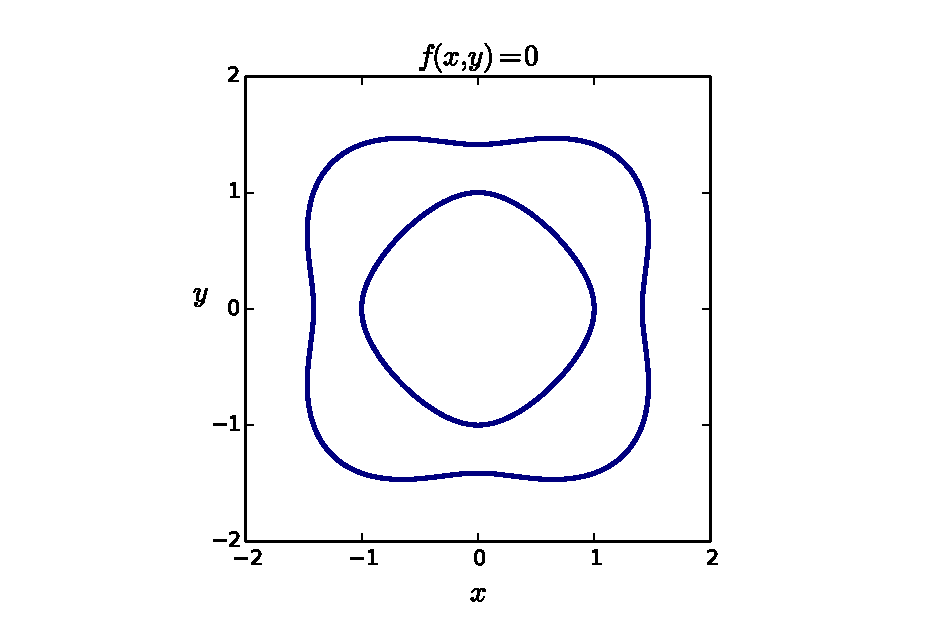
\includegraphics[width=\textwidth]{images/heltonvinnikov.eps}
  \caption{A real plot of the Helton-Vinnikov curve $f(x,y) = x^{4} +
    x^{2} y^{2} - 3 x^{2} + y^{4} - 3 y^{2} + 2$. The region bounded by
    the innermost oval is a spectrahedron.}
  \label{fig: spectrahedron}
\end{figure}

In some applications, it is preferred to have the matrices $A,B,C$ be
real when the curve $F$ is real. The representations important to
studying spectrahedra also require that the linear matrix representation
is a {\it real definite representation}; that is, that the span of
$A,B,$ and $C$ contain a real positive definite matrix. Plaumann,
Sturmfels, and Vinzant \cite{PSV10} study several approaches to
computing real definite matrices of Helton--Vinnikov curves.

The approach chosen by Helton and Vinnikov gives a positive definite
linear matrix representation of a Helton-Vinnikov curve in terms of
theta functions and the Schottky--Klein prime form.

\begin{theorem}
{\bf (Helton--Vinnikov)} Let $C : f(x,y,z) = 0$ be a real homogeneous
curve of degree $d$ with $f(1,0,0) = 0$ and assume
\begin{enumerate}
  \item $C$ is a Helton--Vinnikov curve with the point $f(1,0,0) = 0$
    inside the innermost oval,
  \item the $d$ real intersection points with the line $\{z = 0\}$ are
    distinct non-singular points $Q_1,\ldots,Q_d$ with coordinates $Q_i
    = (-\beta_i : 1 : 0), \beta_i \neq 0$,
  \item $\delta$ is an even theta characteristic with
    $\theta[\delta](0,\Omega) \neq 0$.
\end{enumerate}
Then,
\[
    f(x,y,z) = \det \left( Ix + By + Cz \right),
\]
where $I$ is the $d \times d$ identity matrix, $B =
\text{diag}(\beta_1,\ldots,\beta_d)$, and $C$ is a real symmetric matrix
with diagonal entries
\[
    c_{ii} = \beta_i
    \frac{\partial_z f(-\beta_i,1,0)}{\partial_y f(-\beta_i,1,0)},
\]
and off-diagonal entries
\[
    c_{jk} = \frac{\beta_k - \beta_j}{\theta[\delta](0,\Omega)}
    \frac{\theta[\delta](A(Q_k) - A(Q_j))}{E(Q_j,Q_k)},
\]
where $E : X \times X \to \CC^g$ is the Schottky--Klein prime form.
\end{theorem}

The calculation of linear matrix representations of Helton--Vinnikov
curves is an excellent application of the Schottky--Klein prime form and
I aim to provide an algorithm for doing so.


%------------------------------------------------------------------------------
\subsection{The Constructive Schottky Problem}
%------------------------------------------------------------------------------

As mentioned, the KP equation provides a means for determining if a
Riemann matrix $\Omega \in \hh_g$ comes from the period matrix of some
Riemann surface $X$. The question can be asked, can we find a curve $C :
f(x,y) = 0$ producing this period matrix. This question is called the
Constructive Schottky Problem. That is,
\begin{quote}
  Given a Riemann matrix $\Omega \in \hh_g$ can we find a curve $C :
  f(x,y) = 0$ with $\Omega$ as its period matrix?
\end{quote}
This is a long term endeavor. Regardless, I look to examine possible
avenues for addressing this problem.


%%%%%%%%%%%%%%%%%%%%%%%%%%%%%%%%%%%%%%%%%%%%%%%%%%%%%%%%%%%%%%%%%%%%%%%%%%%%%%%
\section{Bibliography}
%%%%%%%%%%%%%%%%%%%%%%%%%%%%%%%%%%%%%%%%%%%%%%%%%%%%%%%%%%%%%%%%%%%%%%%%%%%%%%%


\bibliographystyle{amsplain}
\bibliography{general-exam}


%%%%%%%%%%%%%%%%%%%%%%%%%%%%%%%%%%%%%%%%%%%%%%%%%%%%%%%%%%%%%%%%%%%%%%%%%%%%%%%
\end{document}
%%%%%%%%%%%%%%%%%%%%%%%%%%%%%%%%%%%%%%%%%%%%%%%%%%%%%%%%%%%%%%%%%%%%%%%%%%%%%%%
